\documentclass[10pt,a4paper,twocolumn]{article}
\usepackage[T1]{fontenc}
\usepackage[utf8]{inputenc}
\usepackage{lmodern}
\usepackage[ngerman]{babel}
\usepackage[margin=2cm,columnsep=0.8cm]{geometry}
\usepackage{microtype}
\usepackage{graphicx}
\usepackage{booktabs}
\usepackage{caption}
\usepackage{subcaption}
\usepackage[round,authoryear]{natbib}
\usepackage[hidelinks]{hyperref}
\newcommand{\gene}[1]{\textit{#1}}
\captionsetup{font=small,labelfont=bf}
\setlength{\parindent}{1em}

\title{Variantenanalyse zweier humaner Gesamtgenome (NA12878 und NA12877): von den Rohdaten zu annotierten ClinVar-Kandidaten und einem Elternvergleich}
\author{Karim Andjar\\[2pt]\small Masterstudiengang Bioinformatik und Systembiologie, Justus-Liebig-Universit\"at Gie\ss en}
\date{}

\begin{document}
\twocolumn[
\maketitle
\begin{center}
\begin{minipage}{0.92\textwidth}
\small
\textbf{Zusammenfassung.}
Ich habe f\"ur zwei Proben des Platinum-Genomes-Pedigrees, NA12878 (Mutter, ERR194147) und NA12877 (Vater, ERR194146), jeweils eine Pipeline von den Rohdaten (Illumina-Paired-End, rund 50-fache Tiefe) bis zu annotierten ClinVar-Kandidaten aufgebaut und mit Snakemake umgesetzt: Qualit\"atskontrolle und Trimming (fastp), Mapping (BWA-MEM gegen GRCh38), Duplikatmarkierung (GATK), Variantenbestimmung (HaplotypeCaller) und Annotation (VEP mit ClinVar). Es wurden 4.893.226 (Mutter) und 4.889.622 (Vater) Varianten gefunden. Ein strenger Filter auf \emph{Pathogenic} und \emph{Likely pathogenic} lieferte je 11 Kandidaten. Die Pipeline enth\"alt keinen Variantenfilter; deshalb habe ich die Kandidaten anhand von Allelbalance, Tiefe und Genotypqualit\"at nachgepr\"uft. Dabei fielen vier (Mutter) bzw.\ drei (Vater) Treffer als Artefaktverdacht heraus; es blieben 7 bzw.\ 6 Kandidaten, von denen 3 bzw.\ 4 als belastbar gelten. Der Vergleich beider Genome ergab kein Gen, in dem beide Eltern eine belastbare Variante tragen. Die Ergebnisse sind ClinVar-Annotationen und keine Diagnosen; eine Validierung gegen ein Referenz-Truth-Set steht noch aus.

\medskip
\textbf{Abstract.}
For two samples of the Platinum Genomes pedigree, NA12878 (mother) and NA12877 (father), I built a Snakemake pipeline from raw Illumina paired-end reads (about 50-fold coverage) to ClinVar-annotated candidate variants (fastp, BWA-MEM on GRCh38, GATK MarkDuplicates and HaplotypeCaller, VEP). About 4.89 million variants were called per genome, and a strict filter for \emph{Pathogenic} and \emph{Likely pathogenic} yielded 11 candidates each. Because the pipeline applies no variant filter, candidates were checked by allele balance, depth and genotype quality; 7 (mother) and 6 (father) remained, of which 3 and 4 are considered reliable. No gene carries a reliable candidate in both parents. Results are ClinVar annotations, not diagnoses, and have not yet been validated against a truth set.
\end{minipage}
\end{center}
\vspace{1em}
]

\section{Einleitung}
Die Sequenzierung ganzer Genome liefert pro Person einige Millionen Abweichungen von der Referenz. Nur ein sehr kleiner Teil davon ist klinisch relevant, und ein noch kleinerer Teil l\"asst sich technisch zuverl\"assig nachweisen. Ziel dieser Arbeit war, den gesamten Weg von den Rohdaten bis zu einer \"uberschaubaren Liste annotierter Kandidaten nachvollziehbar und reproduzierbar umzusetzen und kritisch zu pr\"ufen, welche Treffer belastbar sind.

Als Material dienen zwei Genome des Platinum-Genomes-Pedigrees \citep{eberle2017}: NA12878 und NA12877, die im Pedigree als Eltern gef\"uhrt werden. Beide Proben wurden mit derselben Pipeline verarbeitet. Das erlaubt eine Demonstration des Prinzips der Tr\"agerschaftsanalyse: Tragen beide Eltern eine Variante im selben Gen, und wirkt diese rezessiv, so betr\"agt das Risiko f\"ur ein Kind, beide Kopien zu erben, 25~\%; tr\"agt nur ein Elternteil die Variante, ist ein Kind mit 50~\% Wahrscheinlichkeit Tr\"ager. Diese Rechnung ist hier ein Rechenbeispiel auf \"offentlich verf\"ugbaren Daten und keine Risikoabsch\"atzung f\"ur reale Personen.

\section{Material und Methoden}
\subsection{Daten}
Verwendet wurden die Illumina-Paired-End-Daten ERR194147 (NA12878) und ERR194146 (NA12877) mit einer Leselänge von etwa 101~bp. Referenz war GRCh38.

\subsection{Vorverarbeitung und Mapping}
Die Rohdaten wurden mit FastQC \citep{andrews2010} gepr\"uft und mit fastp \citep{chen2018} von Adaptern und Basen schlechter Qualit\"at bereinigt. Das Mapping erfolgte mit BWA-MEM \citep{li2013}, Duplikate wurden mit GATK MarkDuplicates markiert \citep{mckenna2010}. Eine Rekalibrierung der Basenqualit\"aten (BQSR) wurde nicht durchgef\"uhrt.

\subsection{Variantenbestimmung}
Varianten wurden mit dem GATK-HaplotypeCaller \citep{mckenna2010,vanderauwera2013} im Einzelprobenmodus bestimmt. Ein nachgeschalteter Variantenfilter (VQSR oder Hard Filter) ist in der Pipeline nicht enthalten. Die VCF-Dateien sind daher ungefiltert; das Ti/Tv-Verh\"altnis wurde mit bcftools \citep{danecek2021} bestimmt.

\subsection{Annotation und Kandidatenfilter}
Die Annotation erfolgte mit dem Ensembl Variant Effect Predictor (VEP, Release 116; \citealp{mclaren2016}) unter Verwendung von ClinVar \citep{landrum2018}. Als streng gelten Varianten, deren ClinVar-Klassifikation mit \emph{Pathogenic} oder \emph{Likely pathogenic} beginnt; Eintr\"age mit widerspr\"uchlicher Klassifikation z\"ahlen nicht dazu. Die Klassen folgen der \"ublichen Terminologie \citep{richards2015}. Die Pr\"ufsterne (0 bis 4) geben an, wie gut ein ClinVar-Eintrag abgesichert ist (0: keine Pr\"ufkriterien, 1: ein Einreicher, 2: mehrere Einreicher ohne Widerspruch, 3: Expertengremium, 4: Praxisleitlinie).

\subsection{Qualit\"atsklassen der Kandidaten}
Aus dem AD-Feld der VCF-Datei wurde die Allelbalance AB als Anteil der Alt-Reads an allen Reads am Locus berechnet. Ein echter heterozygoter Genotyp liegt nahe 0,5. Die Kandidaten wurden in drei Klassen eingeteilt:
\begin{itemize}
\item \emph{belastbar}: heterozygot mit AB 0,35--0,75, Tiefe (DP) $\geq$ 15 und Genotypqualit\"at (GQ) $\geq$ 30; homozygot (1/1) mit AB $\geq$ 0,85 und denselben Mindestwerten;
\item \emph{unsicher}: alle \"ubrigen F\"alle, ausdr\"ucklich auch Indels mit AB $<$ 0,25, da der AD-Wert bei Indels systematisch zu niedrig ausf\"allt;
\item \emph{Artefaktverdacht}: SNVs mit AB $<$ 0,25 (heterozygot) bzw.\ AB $<$ 0,5 (homozygot); sie werden verworfen.
\end{itemize}
Die Schwellen sind pragmatisch gew\"ahlt und nicht an einem Truth Set optimiert.

\subsection{Workflow und Visualisierung}
Die Pipeline ist mit Snakemake \citep{molder2021} umgesetzt; die Probe wird \"uber die Konfiguration (\texttt{sample}, \texttt{name}) gew\"ahlt. Der Kandidatenfilter, der Elternvergleich und die Abbildungen sind eigenst\"andige Python-Skripte au\ss erhalb von Snakemake. Abbildungen wurden mit Matplotlib \citep{hunter2007} erstellt. Zur Einordnung der Geschlechtschromosomen wurde die Tiefe von X und Y relativ zum Median der Autosomen berechnet.

\section{Ergebnisse}
\subsection{Sequenzierung und Mapping}
Tabelle~\ref{tab:qc} fasst die Qualit\"atskennzahlen beider Proben zusammen. Beide Datens\"atze sind vergleichbar: Nach dem Trimming blieben 97,3~\% (Mutter) bzw.\ 97,4~\% (Vater) der Reads \"ubrig, die Q30-Anteile stiegen auf 93,3~\% bzw.\ 91,8~\%, und 99,7~\% bzw.\ 99,6~\% der Reads lie\ss en sich abbilden. Die Duplikationsrate liegt in beiden F\"allen bei rund 1,2~\%. Die mittlere Tiefe betr\"agt etwa 50-fach, der Median der Autosomen 51-fach (Mutter) bzw.\ 54-fach (Vater). Die relative Tiefe von X und Y (Mutter 0,97 und 0,093; Vater 0,50 und 0,411) entspricht einer weiblichen bzw.\ m\"annlichen Probe und best\"atigt die Zuordnung (Abb.~\ref{fig:cov}).

\begin{table}[t]
\centering
\small
\caption{Qualit\"atskennzahlen der beiden Proben.}
\label{tab:qc}
\begin{tabular}{@{}lrr@{}}
\toprule
 & Mutter & Vater\\
 & NA12878 & NA12877\\
\midrule
Reads vor fastp (Mio.) & 1.574,5 & 1.626,4\\
Reads nach fastp (Mio.) & 1.531,9 & 1.584,4\\
Q30 nach fastp (\%) & 93,3 & 91,8\\
Abgebildet (\%) & 99,74 & 99,60\\
Korrekt gepaart (\%) & 97,93 & 97,66\\
Duplikate (\%) & 1,18 & 1,19\\
Median Tiefe Autosomen & 51$\times$ & 54$\times$\\
Relative Tiefe X / Y & 0,97 / 0,093 & 0,50 / 0,411\\
\bottomrule
\end{tabular}
\end{table}

\begin{figure*}[t]
\centering
\begin{subfigure}[t]{0.48\textwidth}
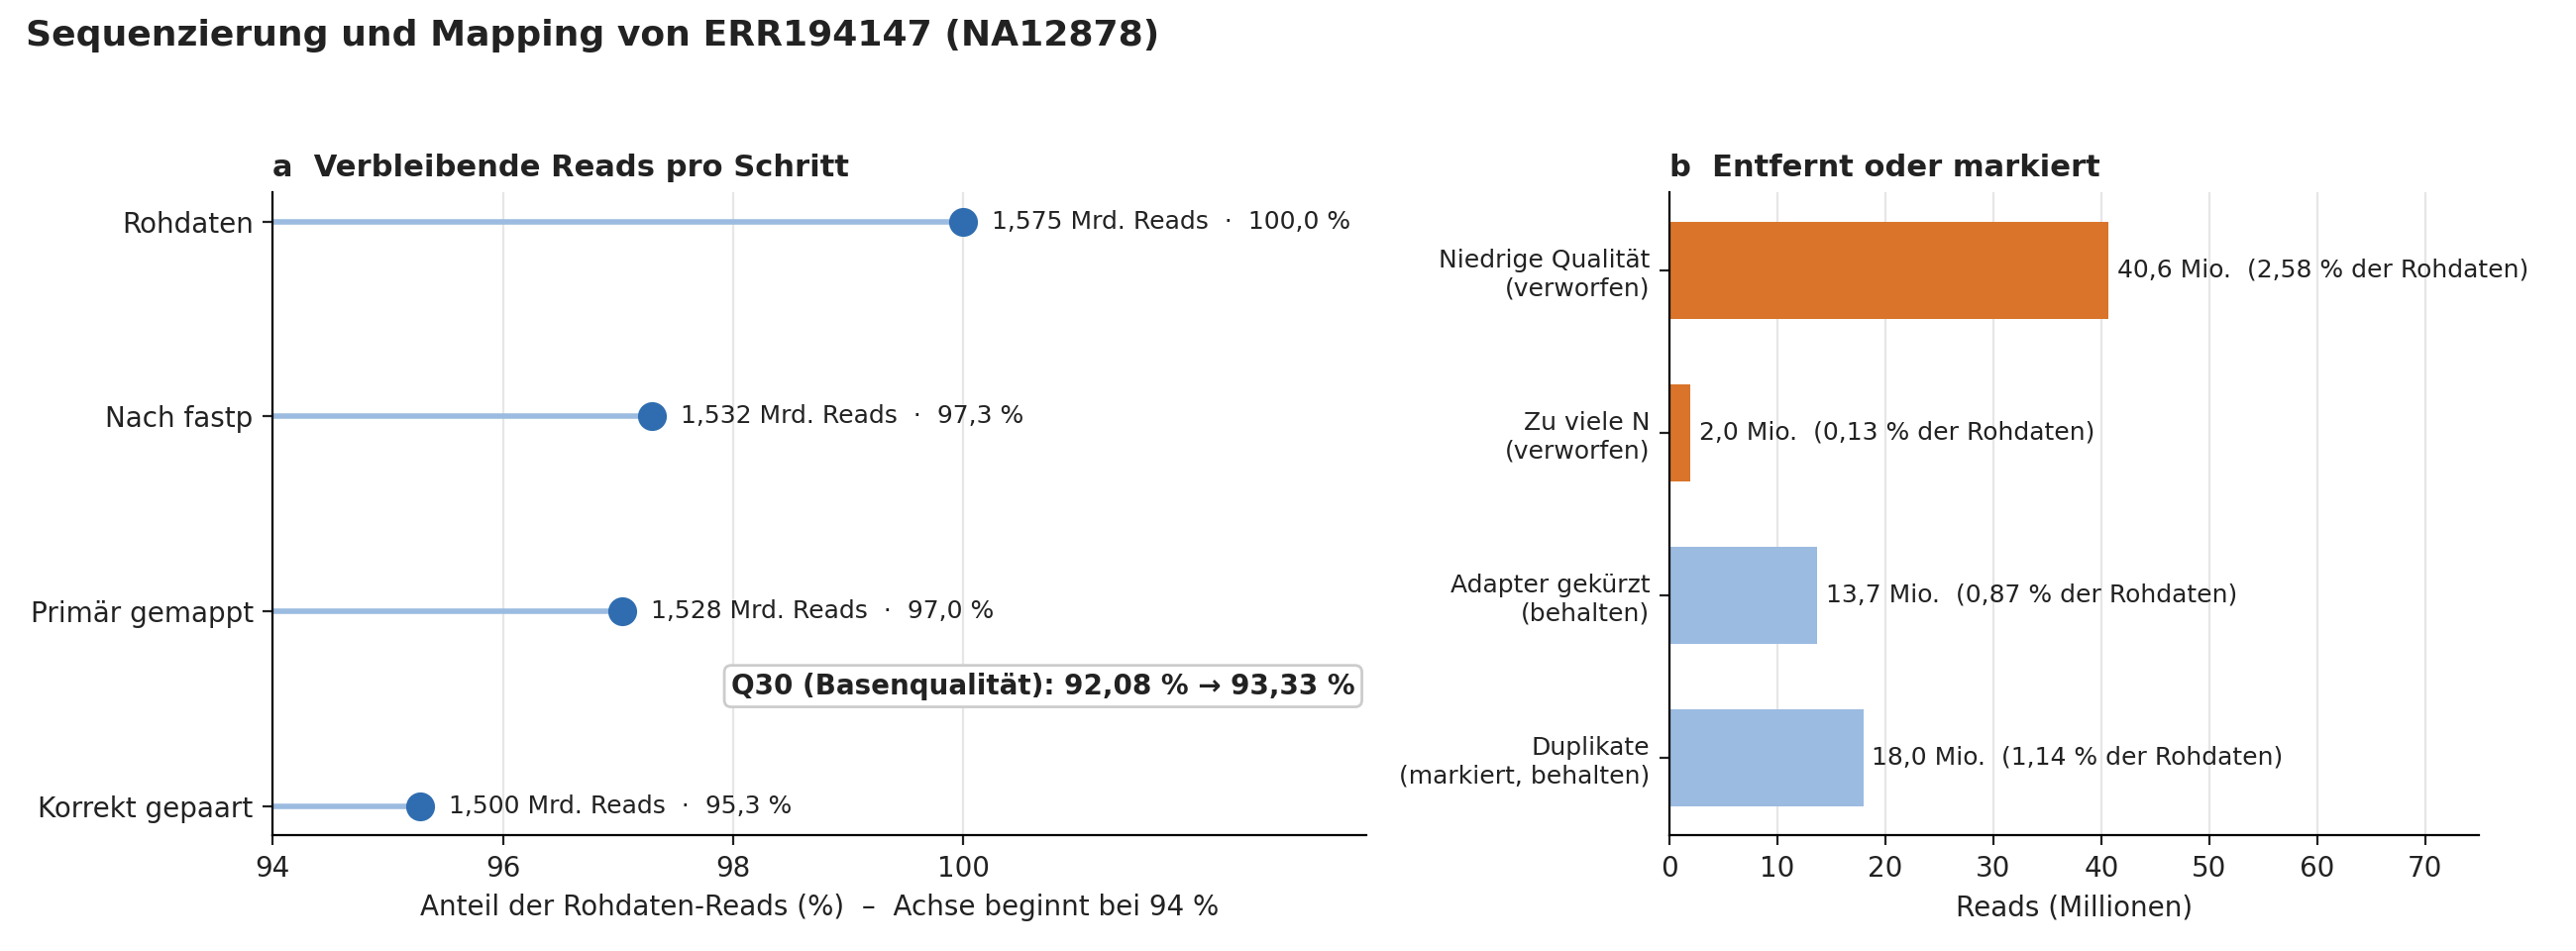
\includegraphics[width=\textwidth]{abbildungen/ERR194147/10_sequenzierung_mapping.png}
\caption{Mutter (NA12878)}
\end{subfigure}\hfill
\begin{subfigure}[t]{0.48\textwidth}
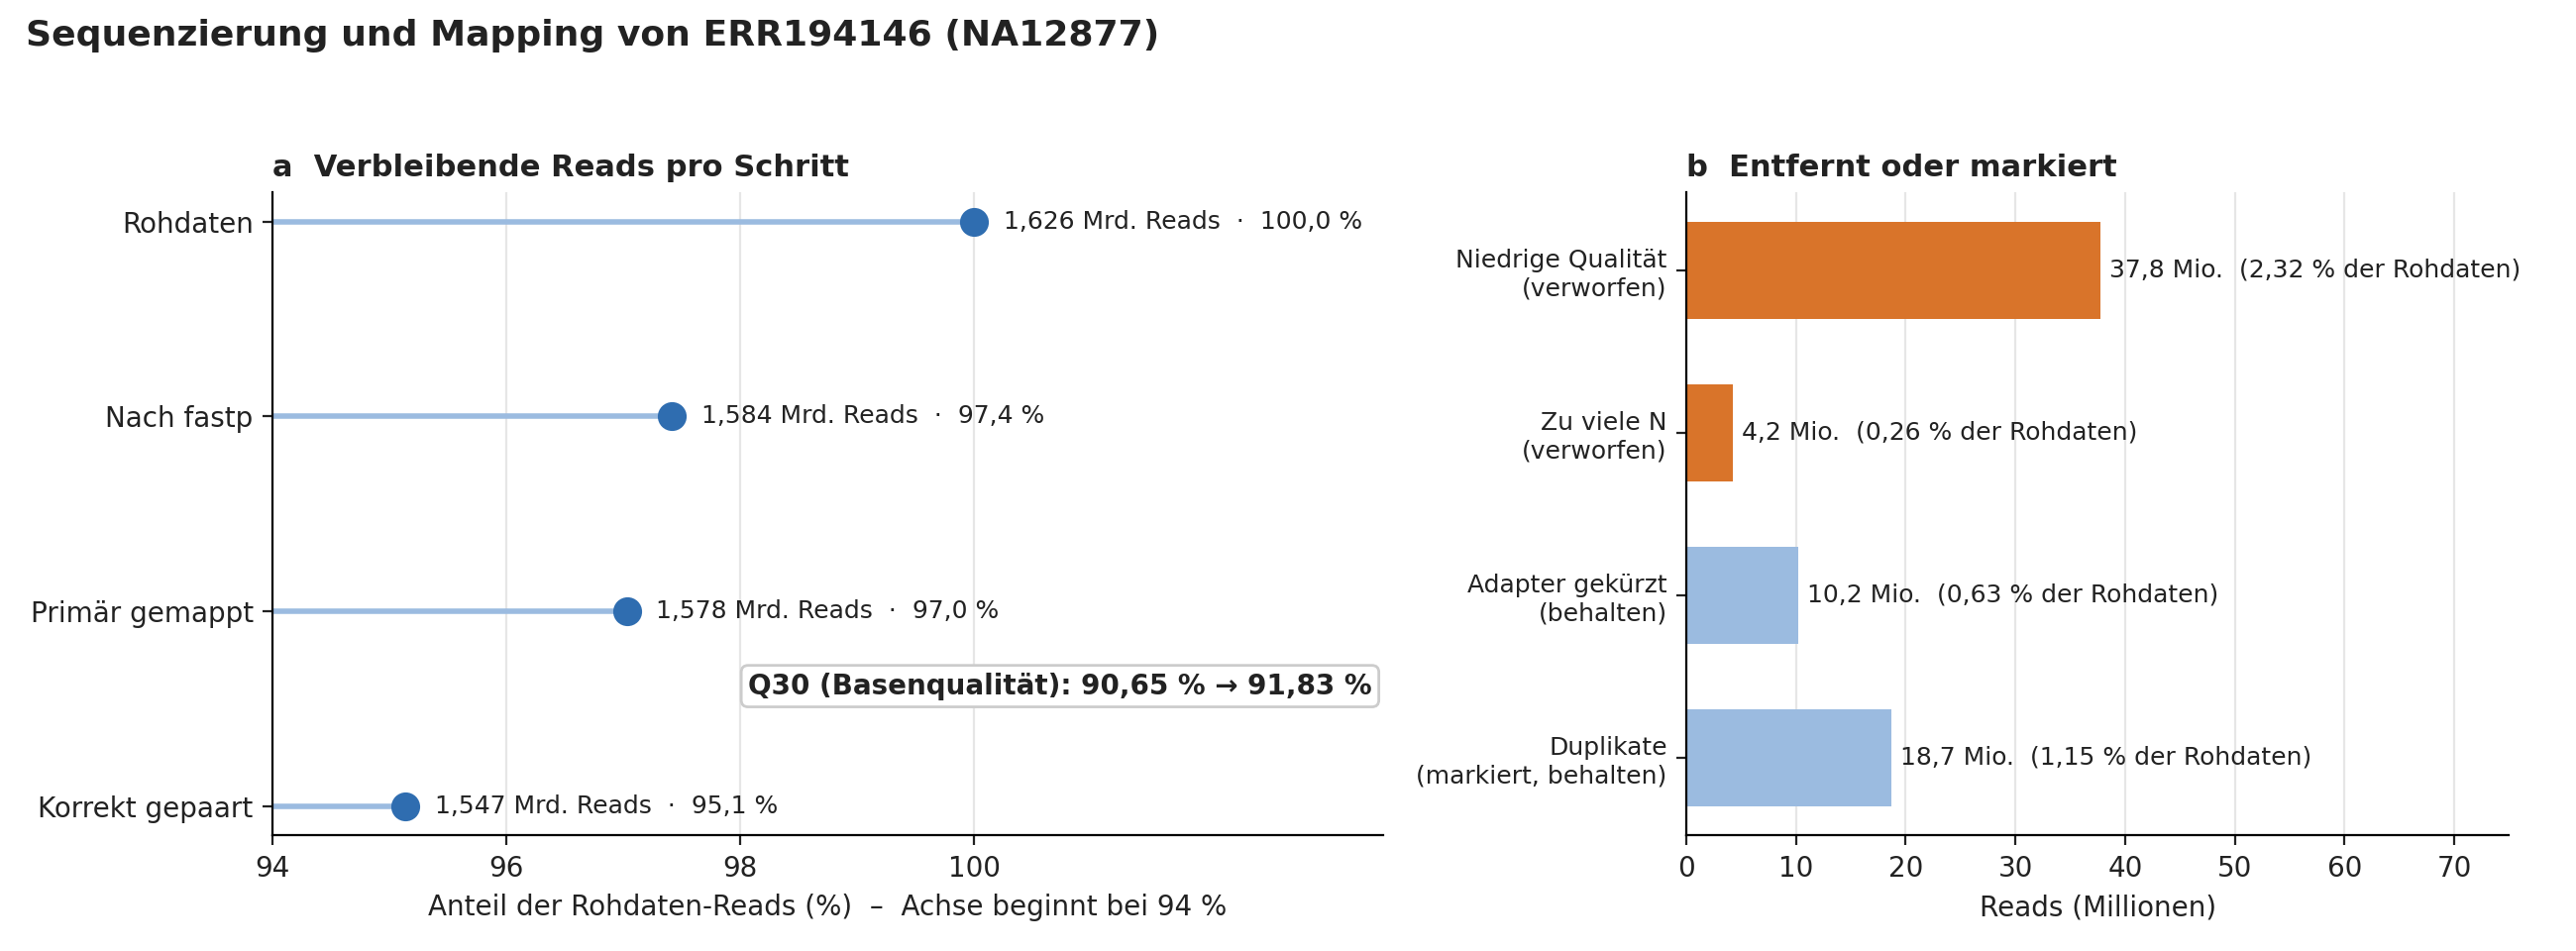
\includegraphics[width=\textwidth]{abbildungen/ERR194146/10_sequenzierung_mapping.png}
\caption{Vater (NA12877)}
\end{subfigure}
\caption{Anteil der Reads nach jedem Verarbeitungsschritt sowie entfernte und markierte Reads.}
\label{fig:seq}
\end{figure*}

\begin{figure*}[t]
\centering
\begin{subfigure}[t]{0.48\textwidth}
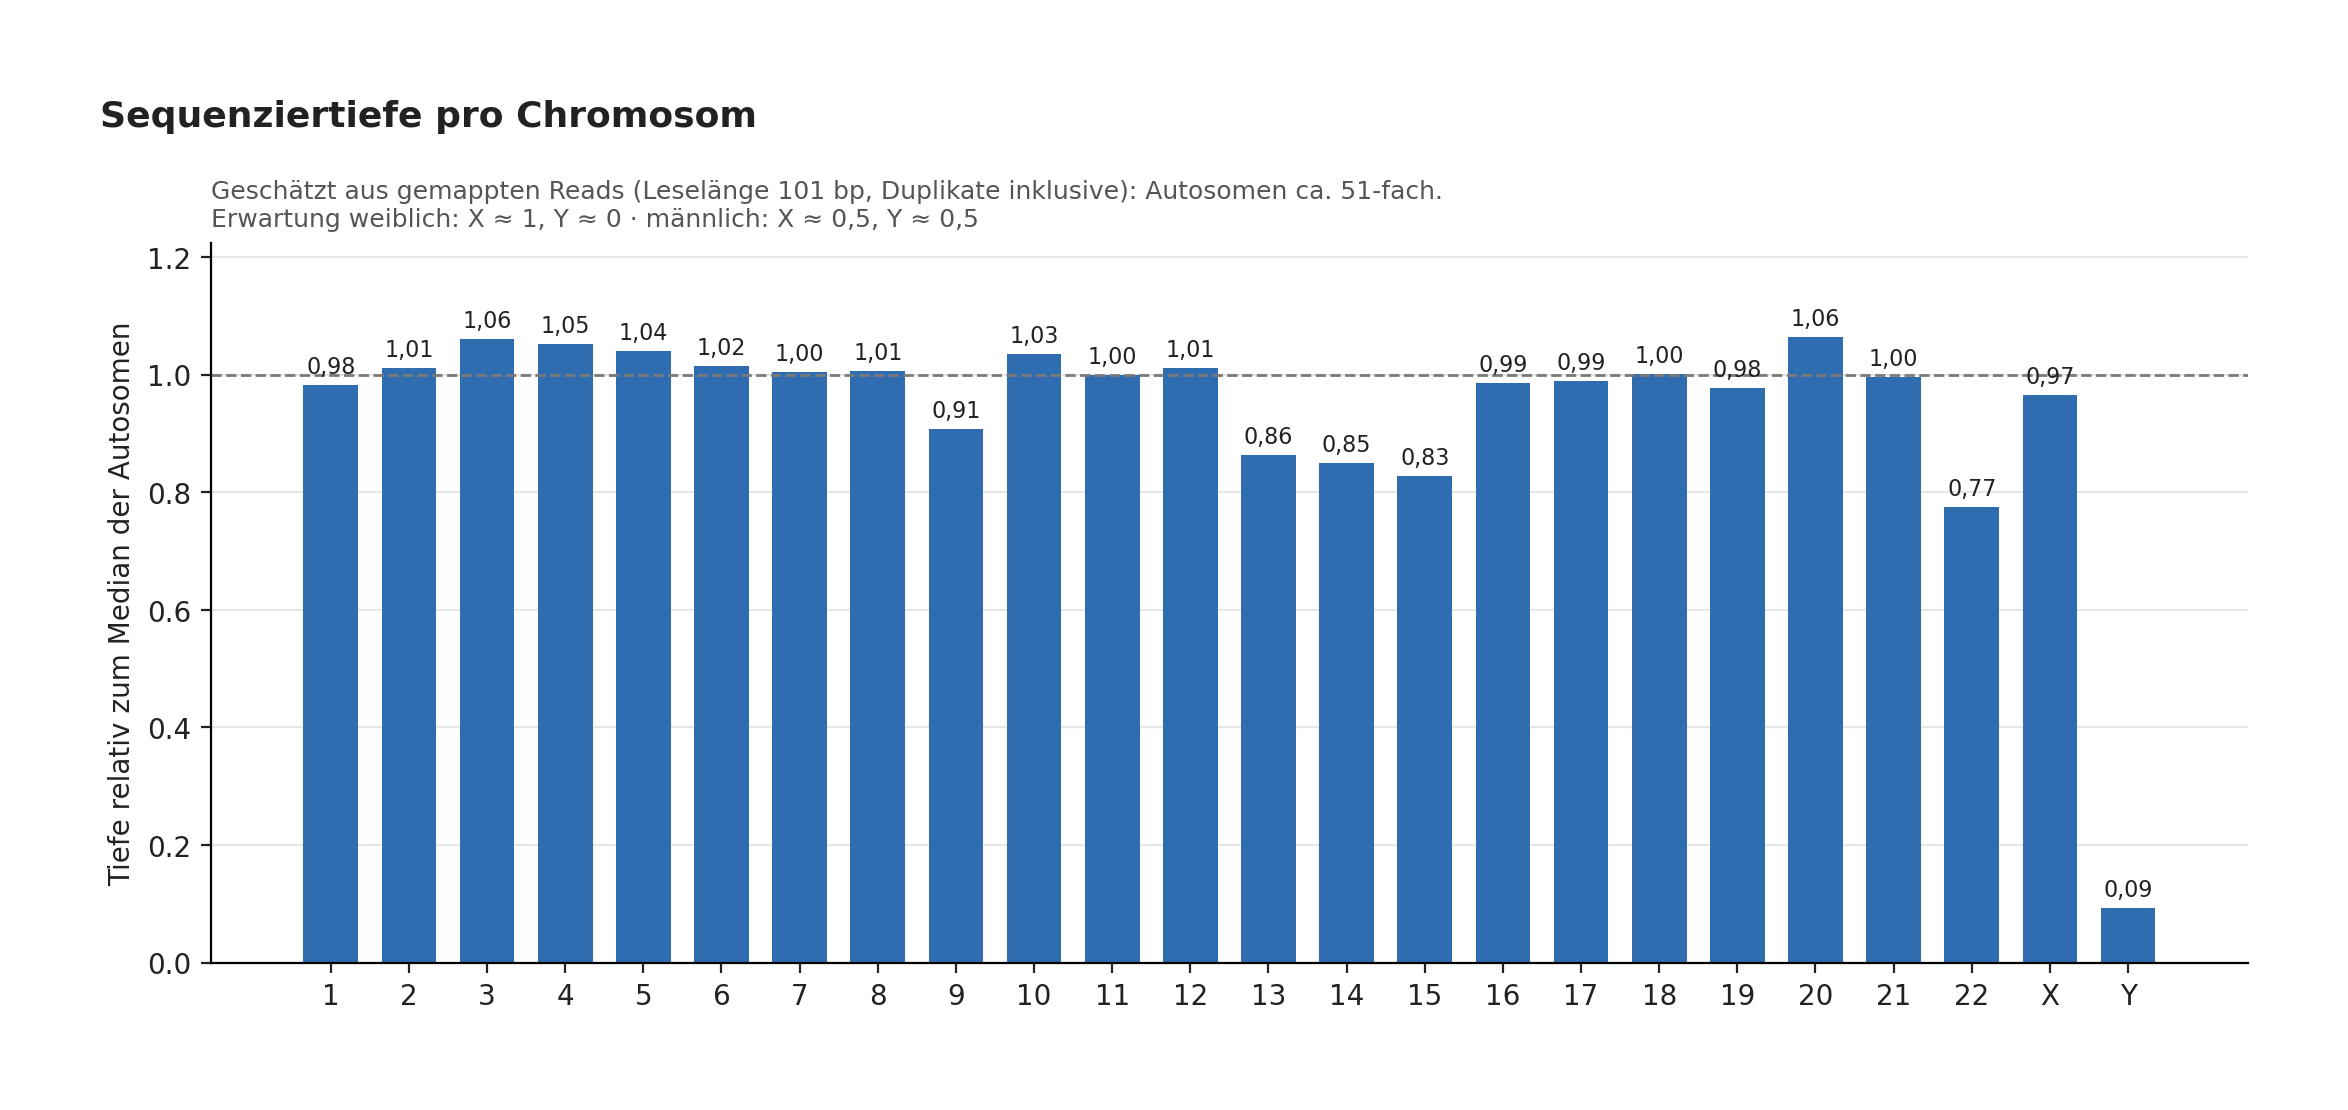
\includegraphics[width=\textwidth]{abbildungen/ERR194147/9_coverage_chromosomen.png}
\caption{Mutter (NA12878)}
\end{subfigure}\hfill
\begin{subfigure}[t]{0.48\textwidth}
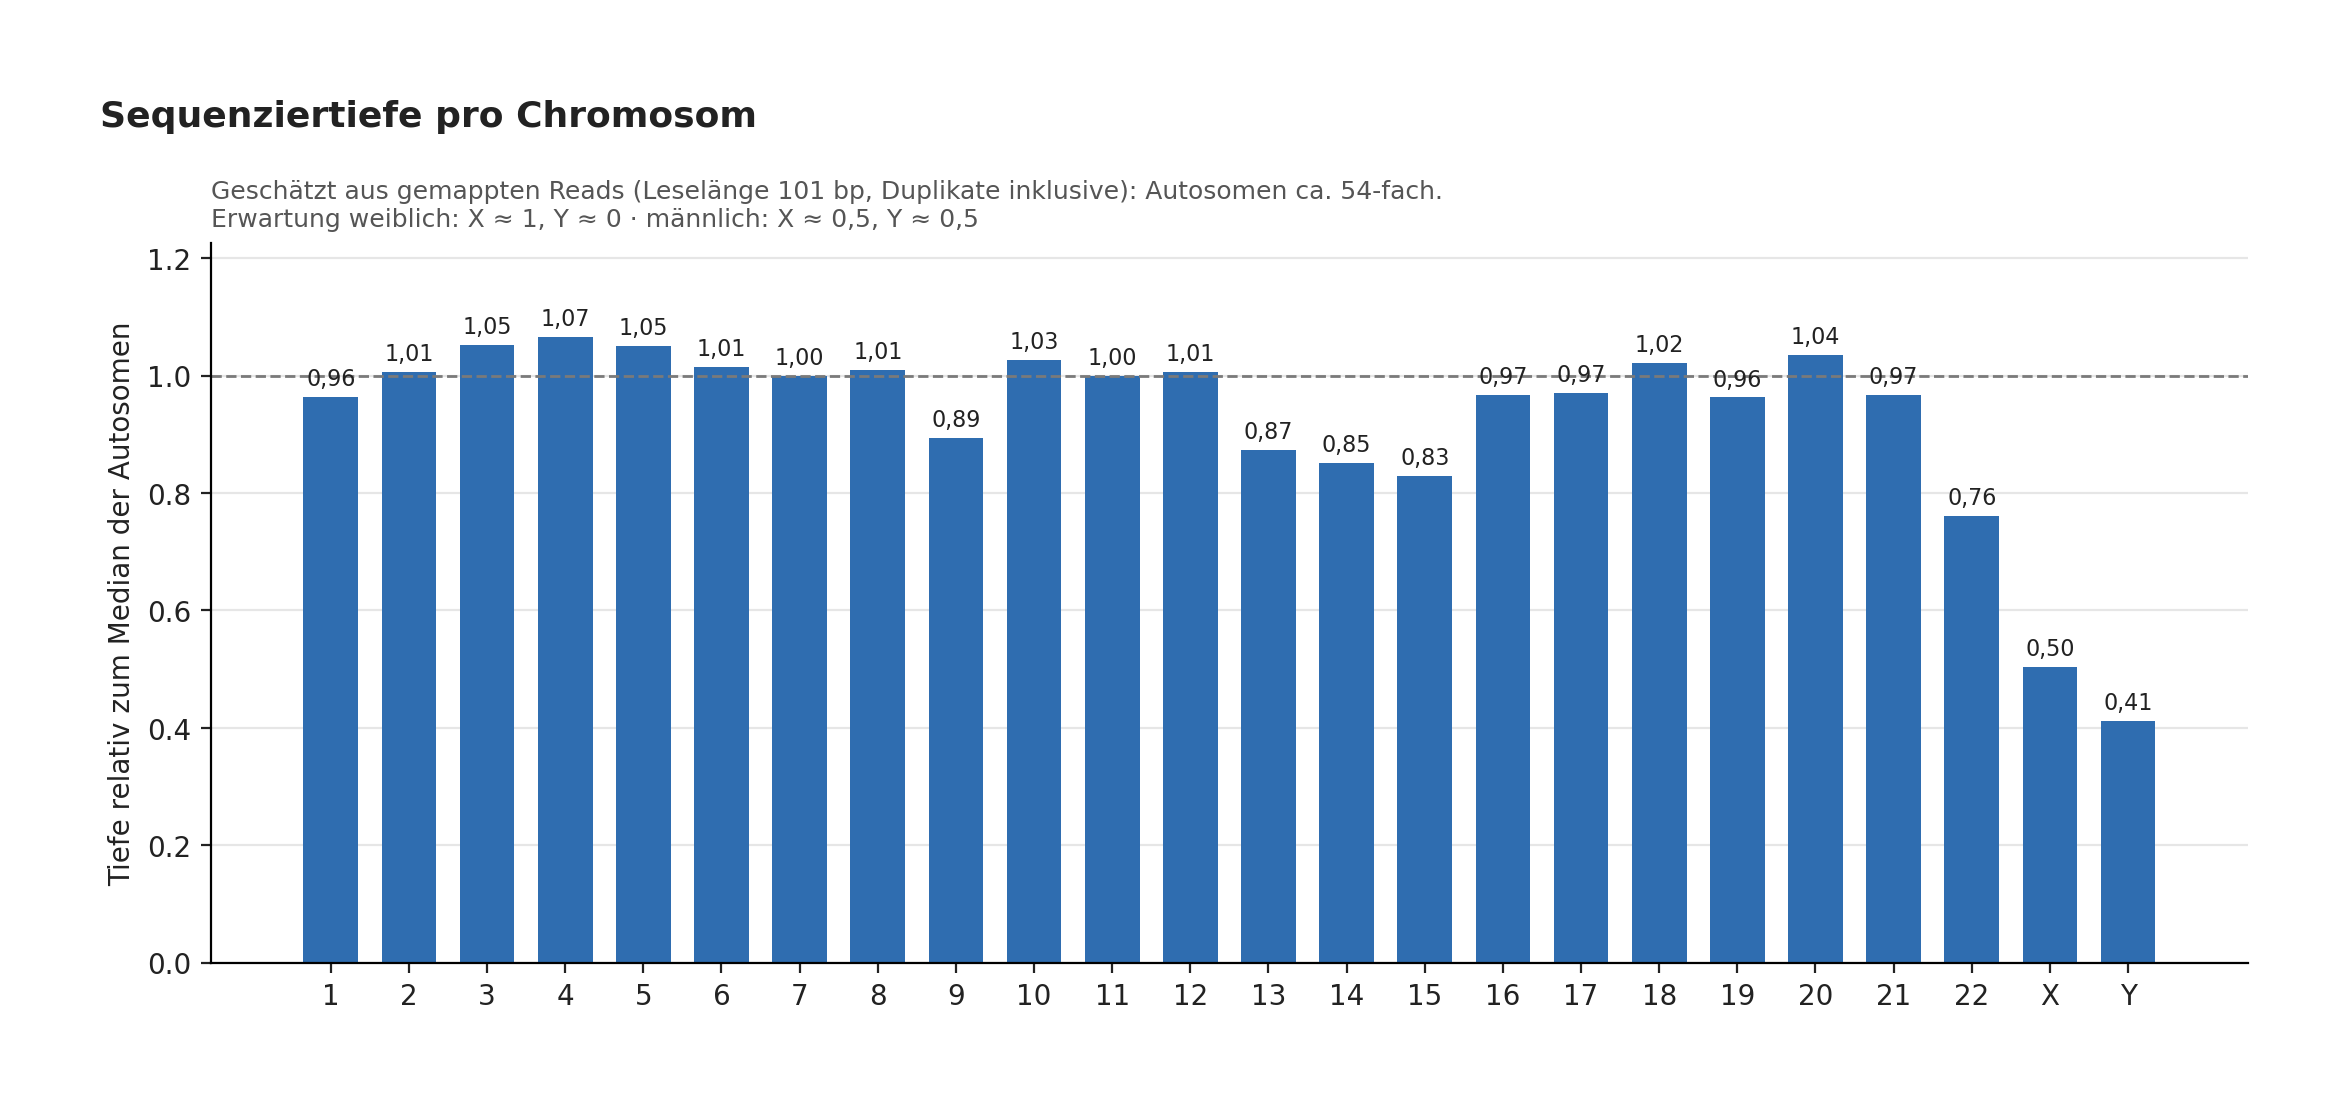
\includegraphics[width=\textwidth]{abbildungen/ERR194146/9_coverage_chromosomen.png}
\caption{Vater (NA12877)}
\end{subfigure}
\caption{Sequenziertiefe pro Chromosom relativ zum Median der Autosomen.}
\label{fig:cov}
\end{figure*}

\subsection{Varianten}
Der HaplotypeCaller lieferte 4.893.226 (Mutter) bzw.\ 4.889.622 (Vater) Varianten (Tab.~\ref{tab:var}, Abb.~\ref{fig:stat}). Das Ti/Tv-Verh\"altnis liegt in beiden Proben bei 1,98 und das Verh\"altnis heterozygoter zu homozygoten Varianten bei 1,70 bzw.\ 1,64, was f\"ur humane Gesamtgenome im \"ublichen Bereich liegt. Auf dem Y-Chromosom wurden in beiden Proben rund 14.000 Varianten gefunden; bei der weiblichen Probe sind sie Mapping-Artefakte aus Sequenzen, die auch auf X oder in Wiederholungen vorkommen, und auch beim m\"annlichen Genom d\"urfte ein Gro\ss teil darauf zur\"uckgehen.

\begin{table}[t]
\centering
\small
\caption{Varianten pro Probe (Chromosomen 1--22, X, Y). Rund 84.000 weitere Varianten liegen auf Contigs.}
\label{tab:var}
\begin{tabular}{@{}lrr@{}}
\toprule
 & Mutter & Vater\\
\midrule
SNVs & 3.970.524 & 3.957.389\\
Insertionen & 372.923 & 381.250\\
Deletionen & 397.247 & 402.146\\
Multiallelisch & 68.136 & 70.438\\
Ti/Tv & 1,98 & 1,98\\
Het/Hom & 1,70 & 1,64\\
\bottomrule
\end{tabular}
\end{table}

\begin{figure*}[t]
\centering
\begin{subfigure}[t]{0.48\textwidth}
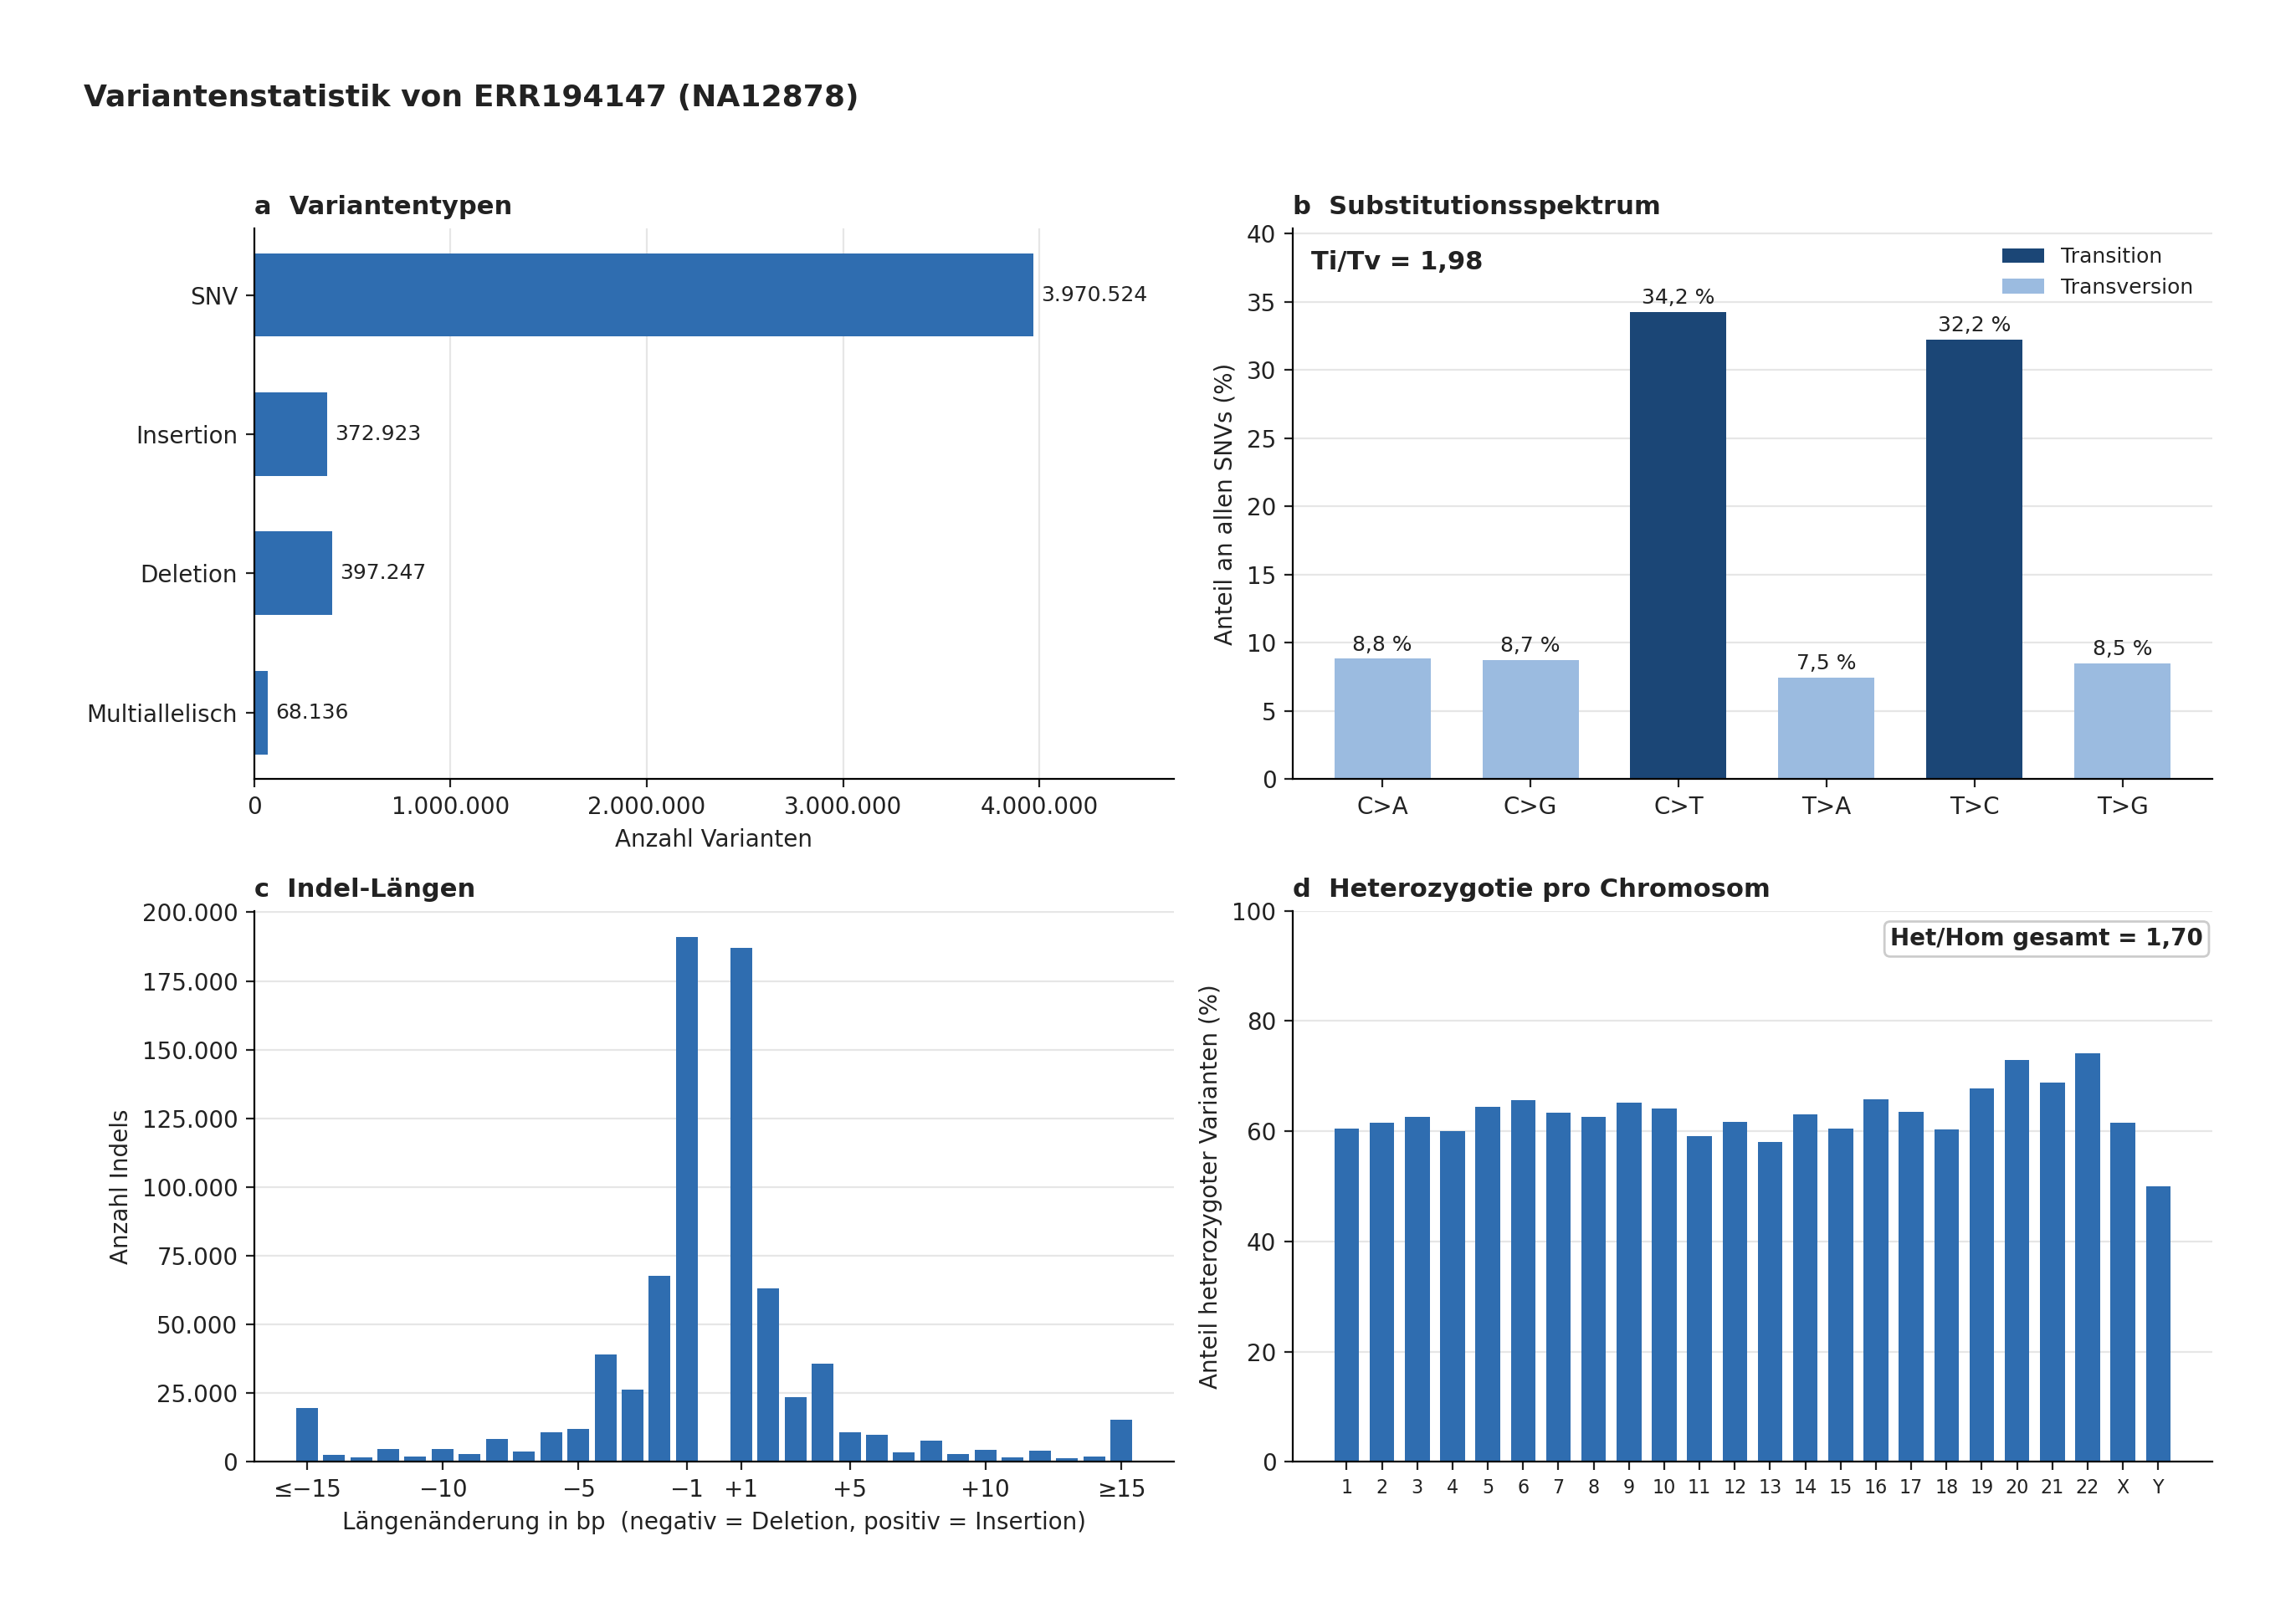
\includegraphics[width=\textwidth]{abbildungen/ERR194147/8_variantenstatistik.png}
\caption{Mutter (NA12878)}
\end{subfigure}\hfill
\begin{subfigure}[t]{0.48\textwidth}
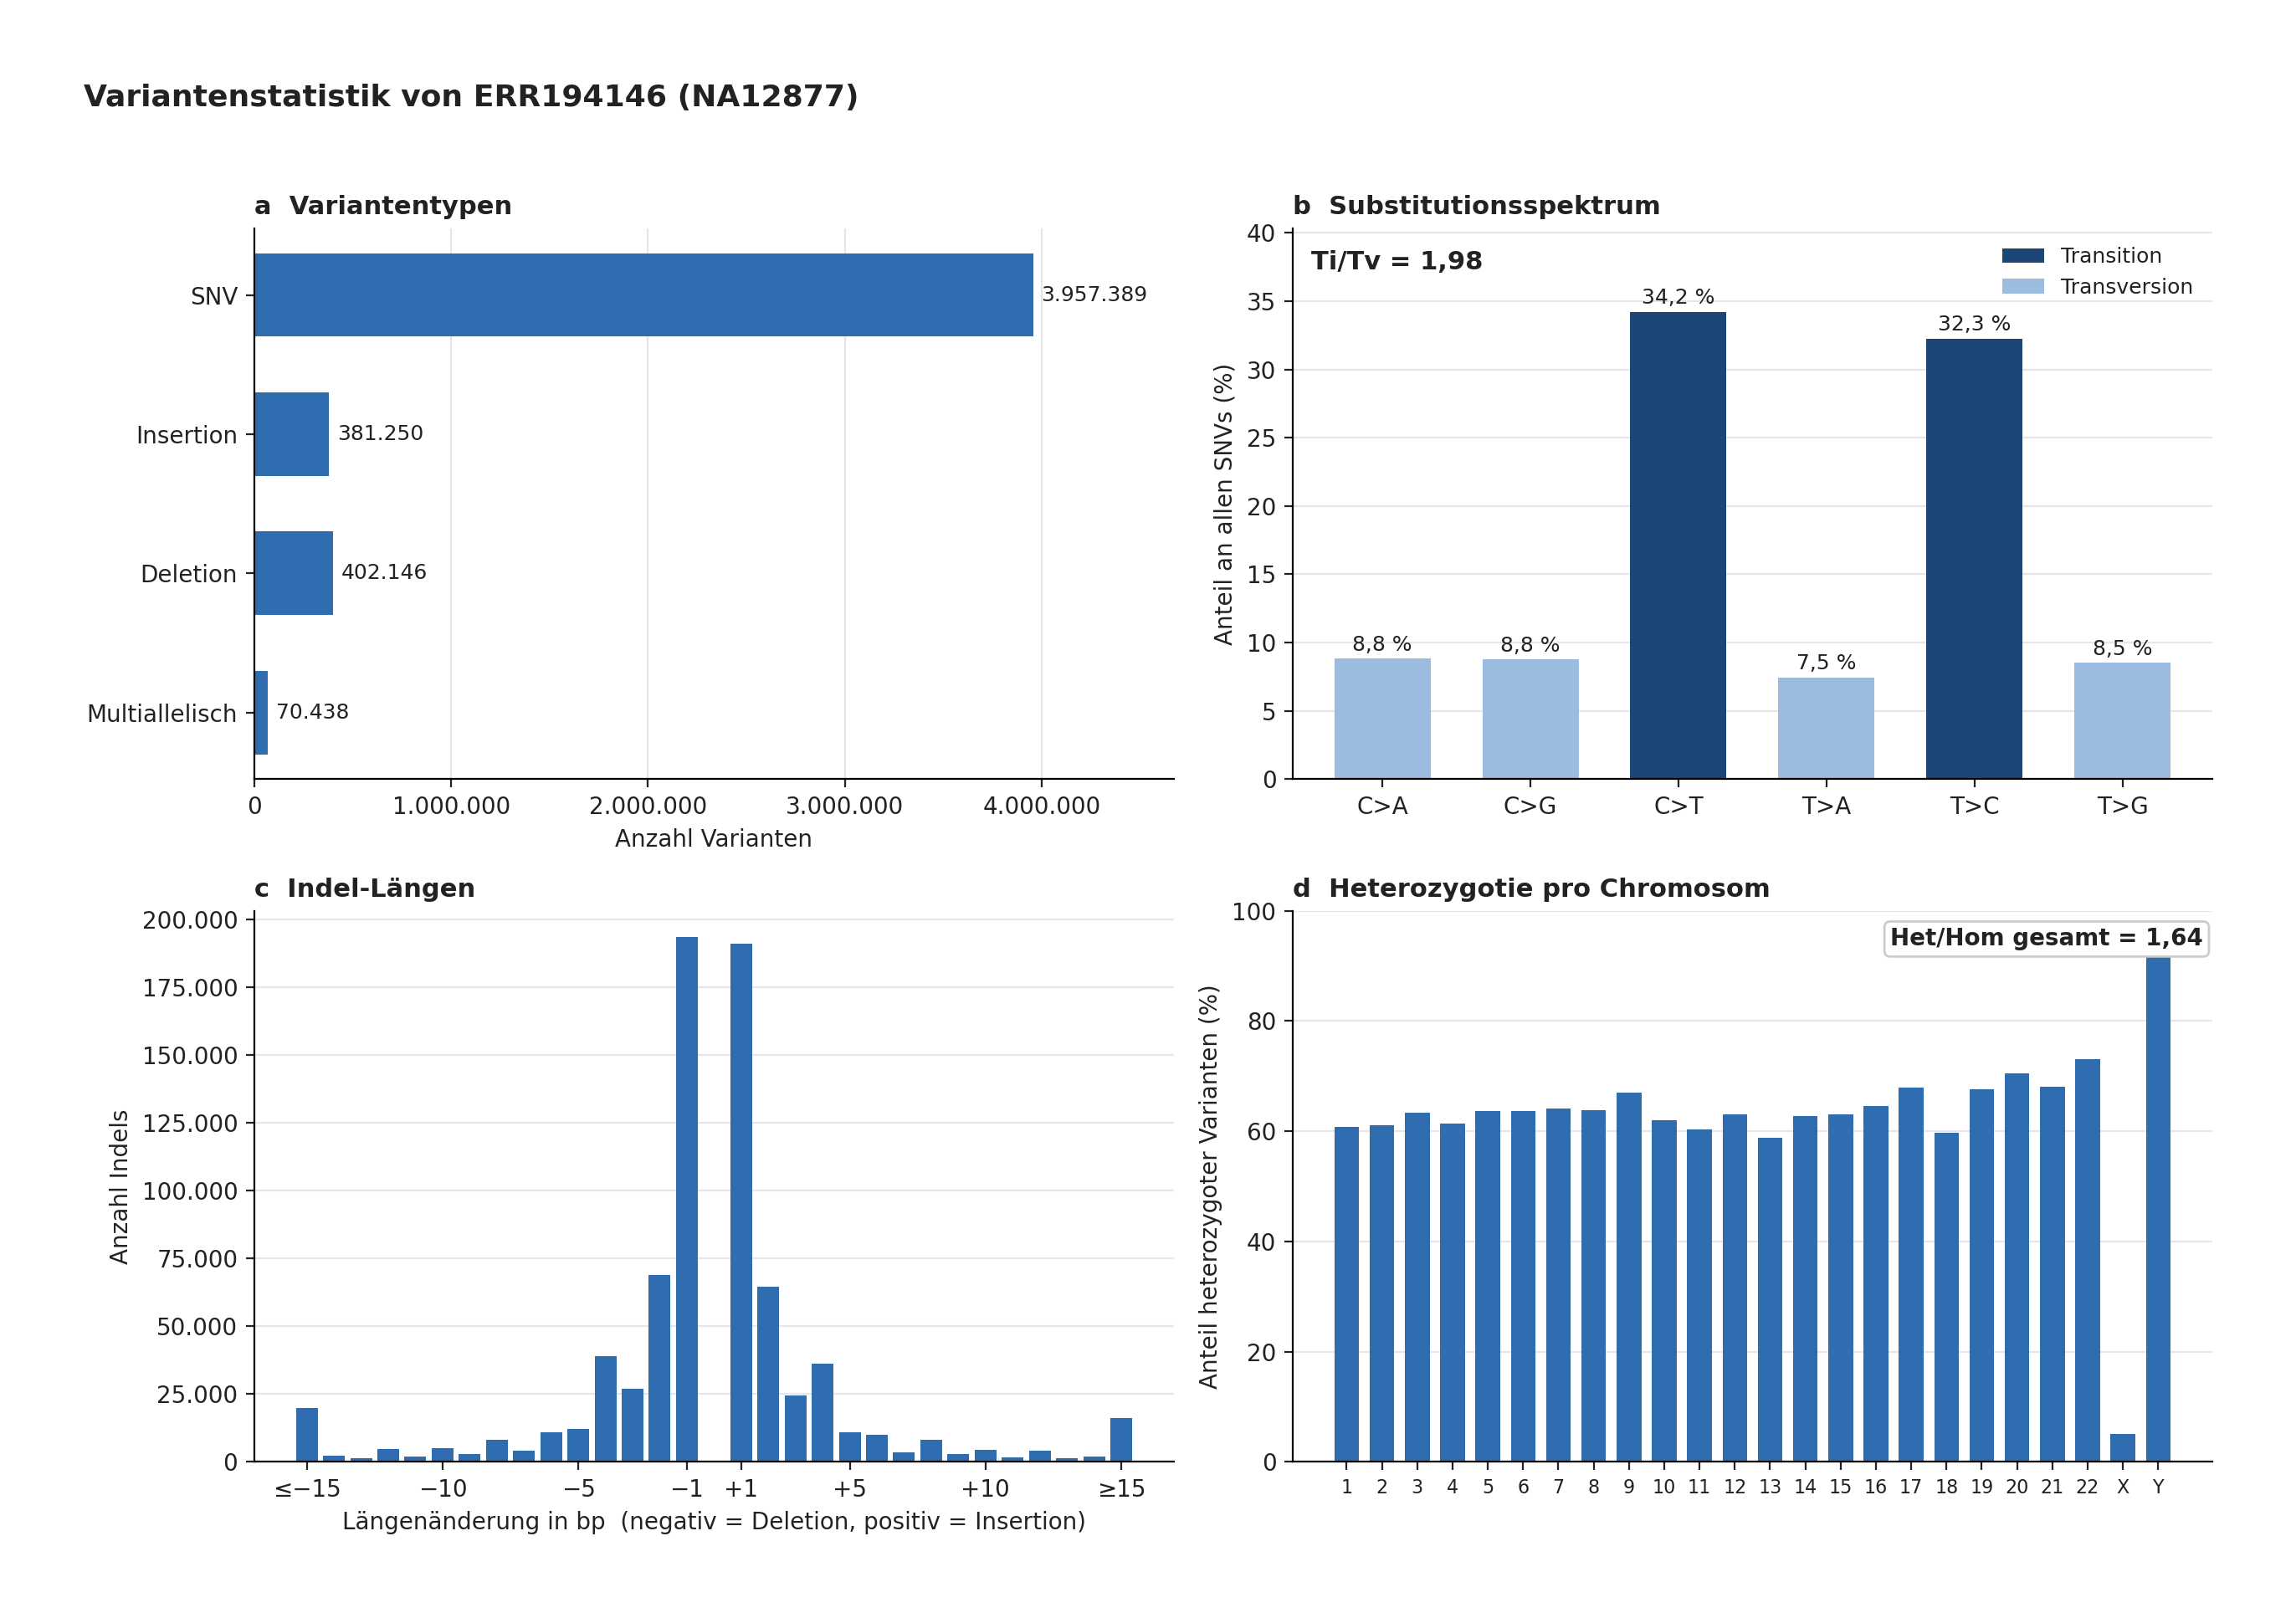
\includegraphics[width=\textwidth]{abbildungen/ERR194146/8_variantenstatistik.png}
\caption{Vater (NA12877)}
\end{subfigure}
\caption{Variantenstatistik: Variantentypen, Substitutionsspektrum mit Ti/Tv, Indel-L\"angen und Anteil heterozygoter Varianten pro Chromosom.}
\label{fig:stat}
\end{figure*}

\begin{figure*}[t]
\centering
\begin{subfigure}[t]{0.48\textwidth}
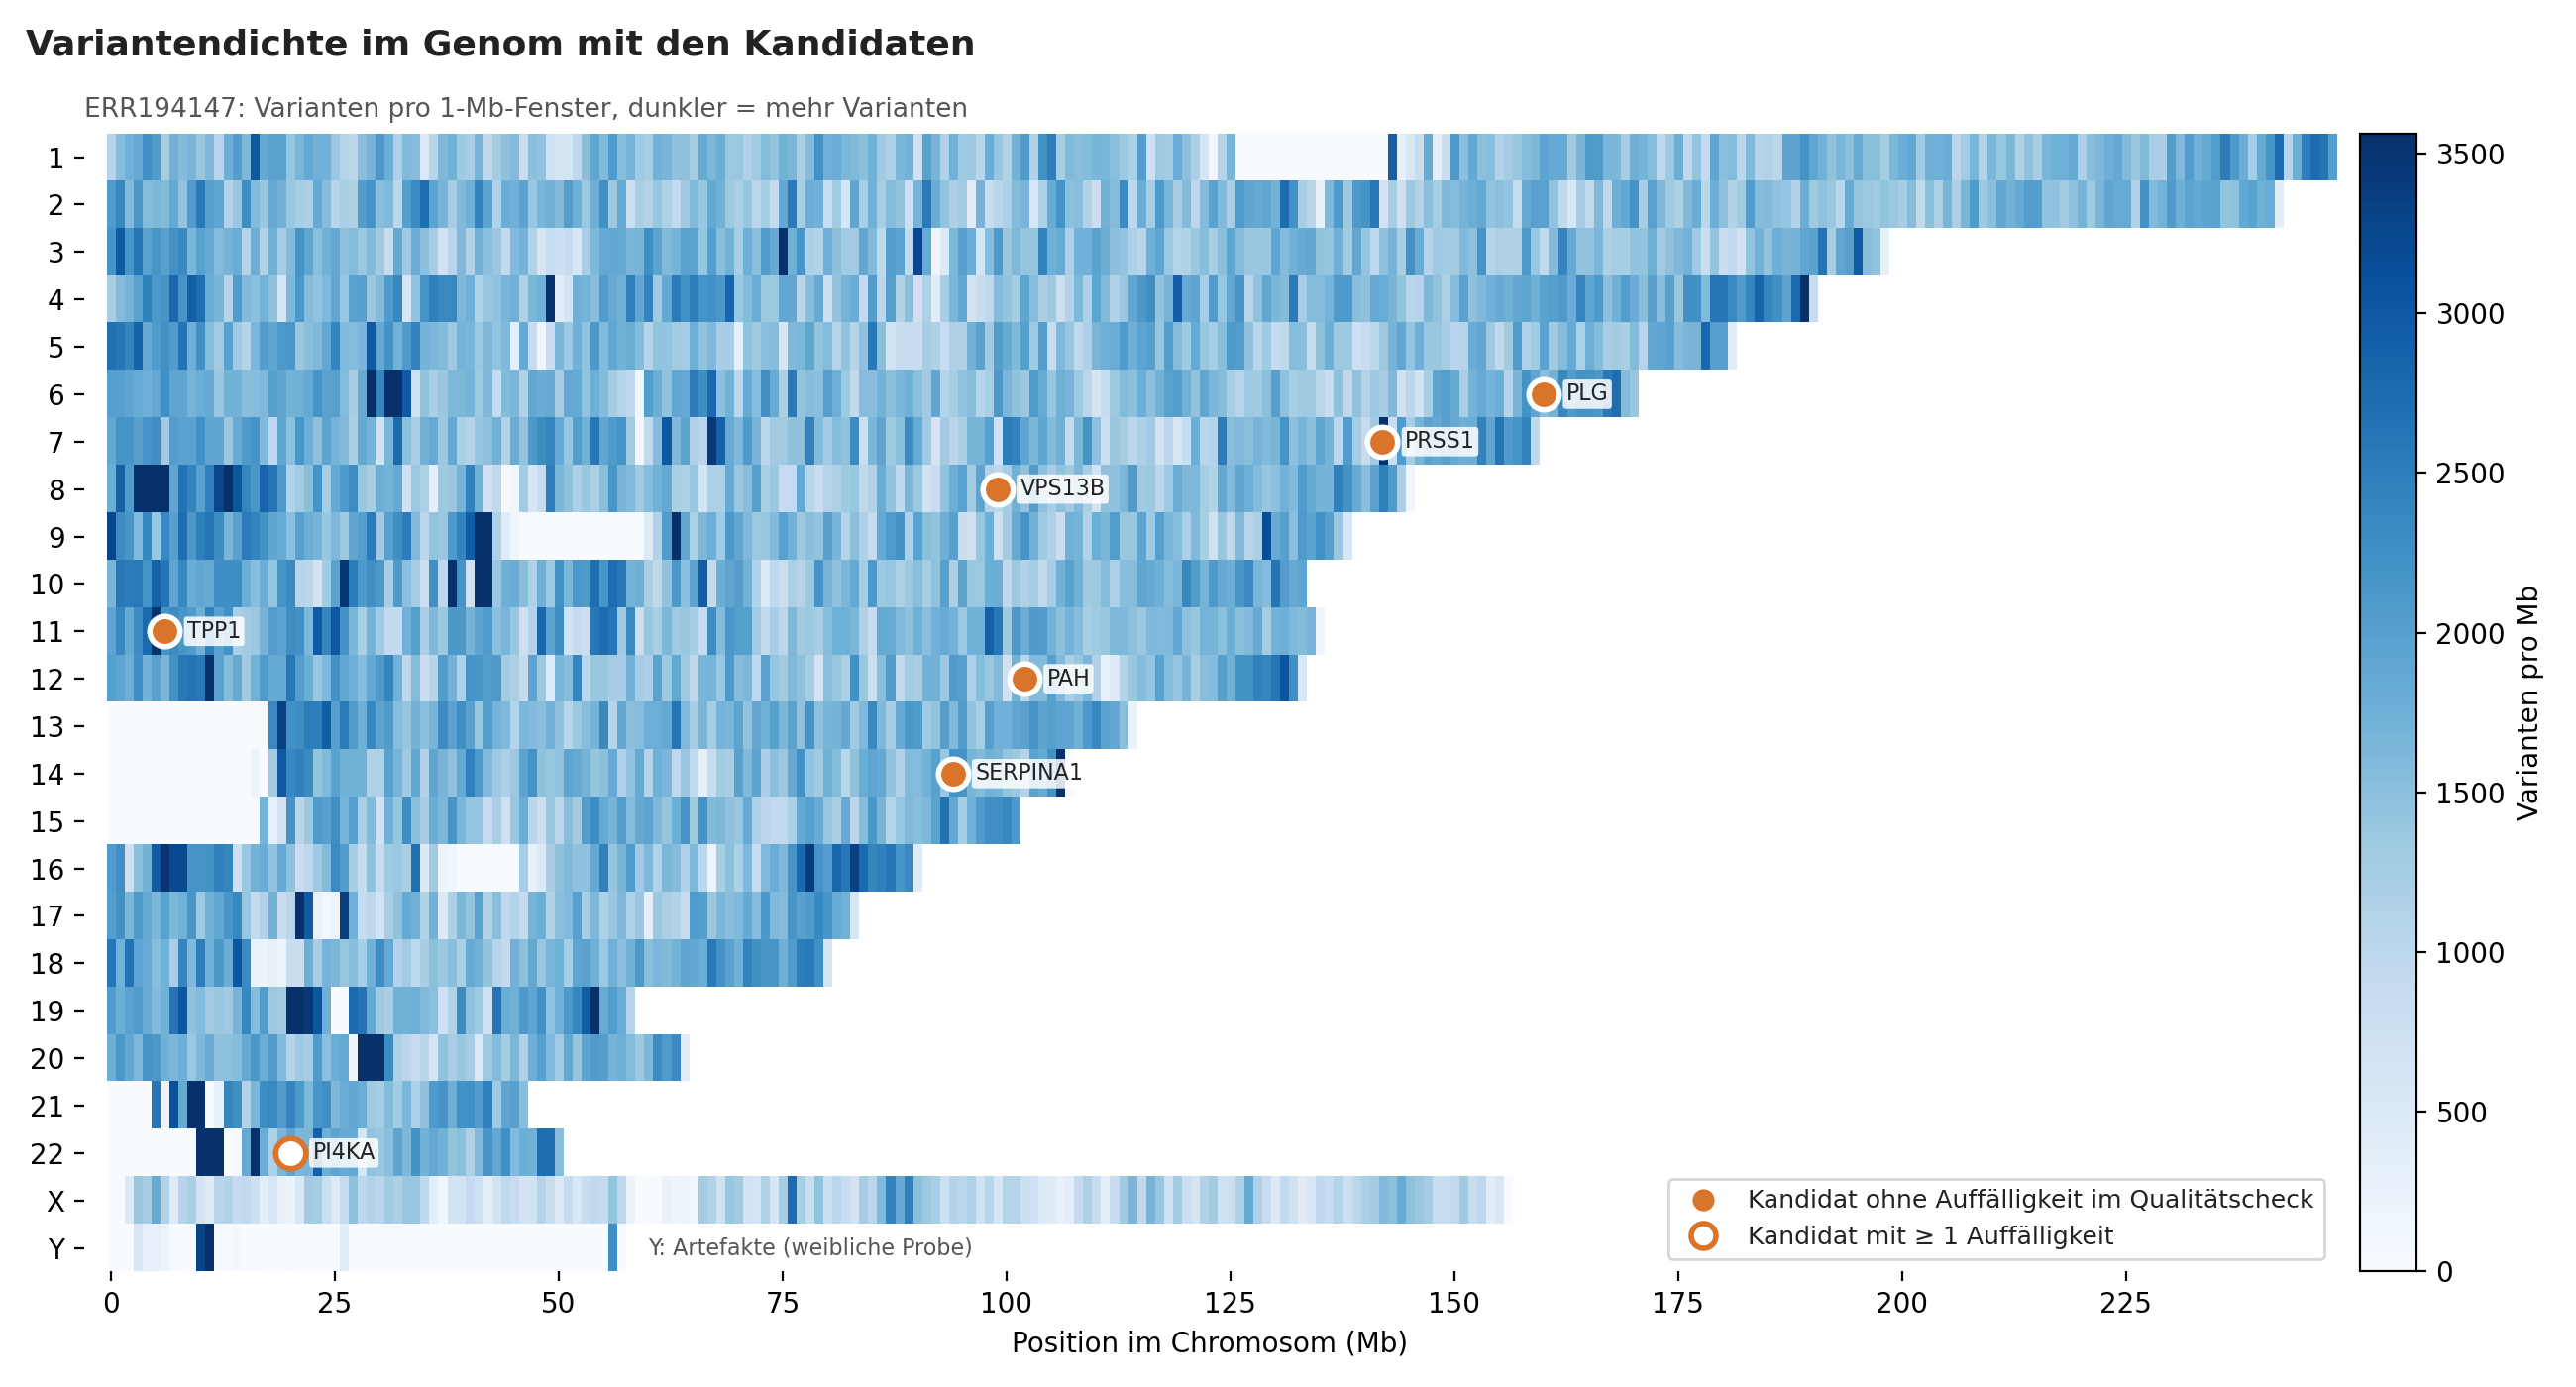
\includegraphics[width=\textwidth]{abbildungen/ERR194147/5_dichte_kandidaten.png}
\caption{Mutter (NA12878)}
\end{subfigure}\hfill
\begin{subfigure}[t]{0.48\textwidth}
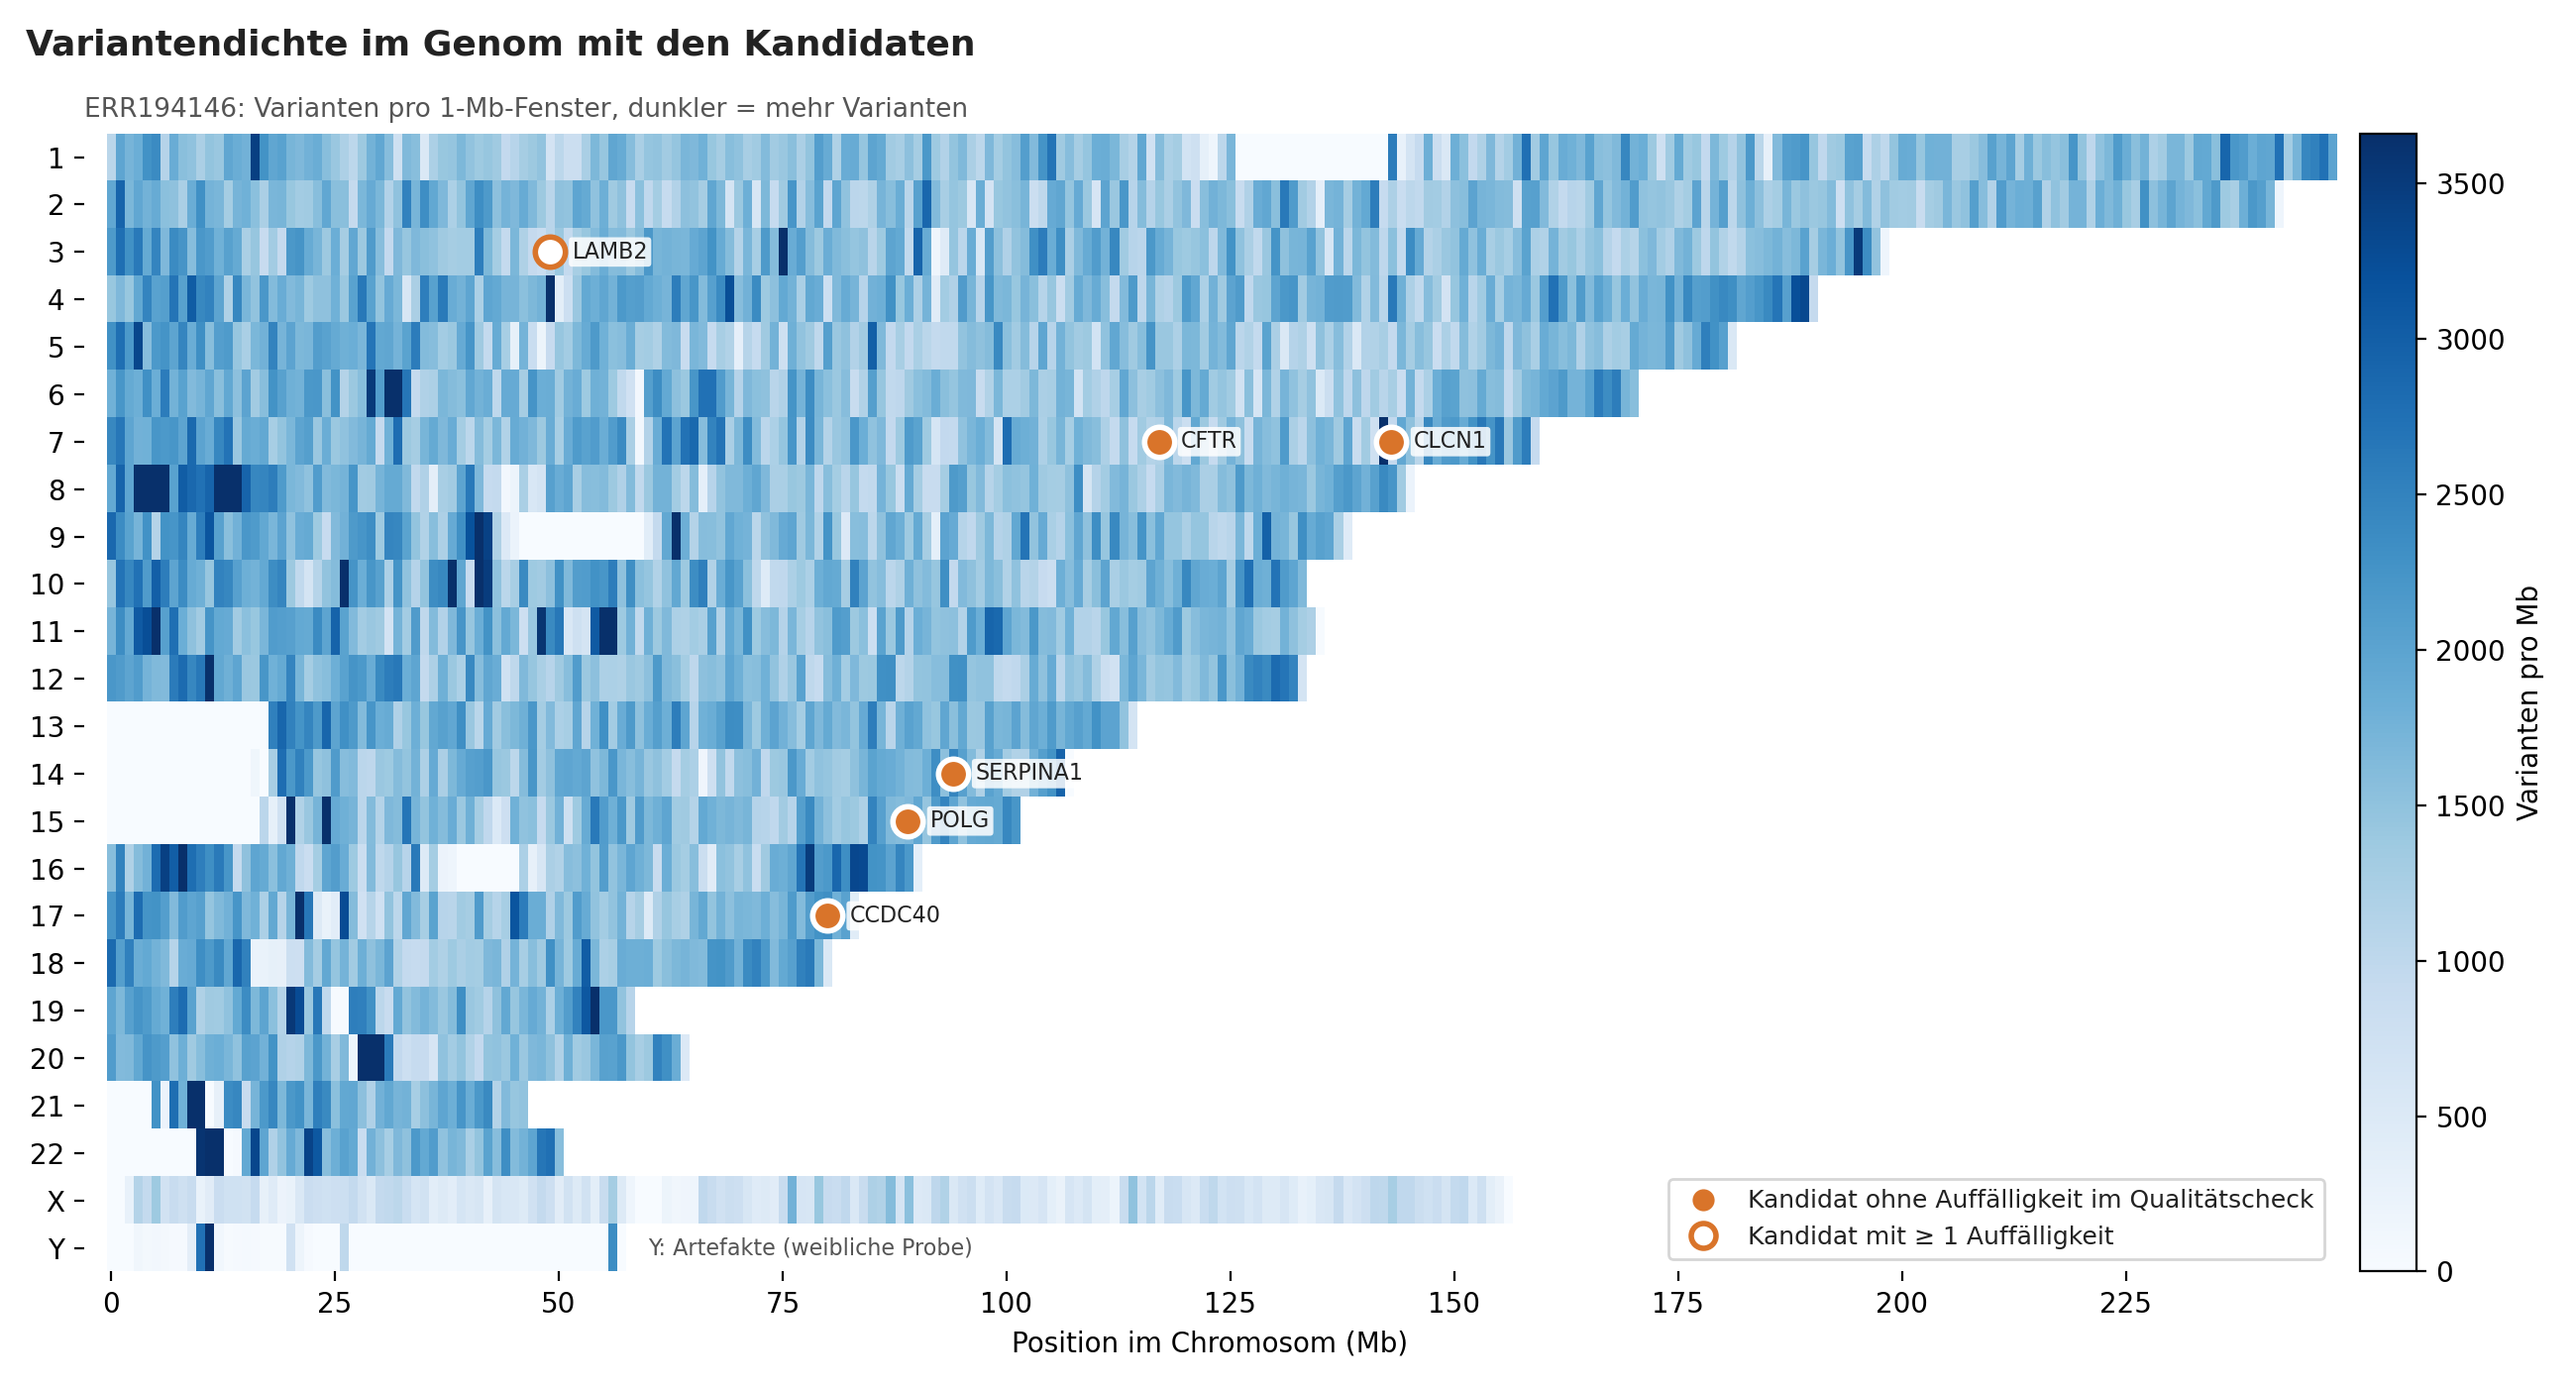
\includegraphics[width=\textwidth]{abbildungen/ERR194146/5_dichte_kandidaten.png}
\caption{Vater (NA12877)}
\end{subfigure}
\caption{Variantendichte pro Megabase und Lage der Kandidaten.}
\label{fig:dichte}
\end{figure*}

\subsection{Annotation und Filtertrichter}
VEP annotierte 4.864.560 (Mutter) bzw.\ 4.864.034 (Vater) Varianten. Die Differenz zu den gerufenen Varianten betr\"agt in beiden Proben etwa 0,6~\%; sie entspricht der Gr\"o\ss enordnung der Varianten auf Contigs, ich habe sie aber nicht vollst\"andig aufgekl\"art. F\"ur rund 44.000 Varianten gab es einen ClinVar-Treffer, \"uberwiegend als \glqq Benign\grqq{} (Tab.~\ref{tab:trichter}). Als pathogen im weiten Sinn blieben 181 bzw.\ 188 Varianten, davon jeweils nur 11 mit eindeutiger Klassifikation; der Rest hat eine widerspr\"uchliche Klassifikation. Beim Vater sind 9 der 11 Treffer proteinver\"andernd, bei der Mutter alle 11. Der anschlie\ss ende Qualit\"atsfilter (Abschnitt~\ref{sec:kand}) reduziert die Liste auf 7 bzw.\ 6 Kandidaten (Abb.~\ref{fig:trichter}).

\begin{table}[t]
\centering
\small
\caption{Filtertrichter pro Probe.}
\label{tab:trichter}
\begin{tabular}{@{}lrr@{}}
\toprule
Stufe & Mutter & Vater\\
\midrule
Varianten gesamt & 4.893.226 & 4.889.622\\
VEP-annotiert & 4.864.560 & 4.864.034\\
mit ClinVar-Eintrag & 44.476 & 43.890\\
pathogen (weit gefasst) & 181 & 188\\
streng (P/LP) & 11 & 11\\
davon proteinver\"andernd & 11 & 9\\
nach Qualit\"atsfilter & 7 & 6\\
\bottomrule
\end{tabular}
\end{table}

\begin{figure}[t]
\centering
\begin{subfigure}[t]{0.49\columnwidth}
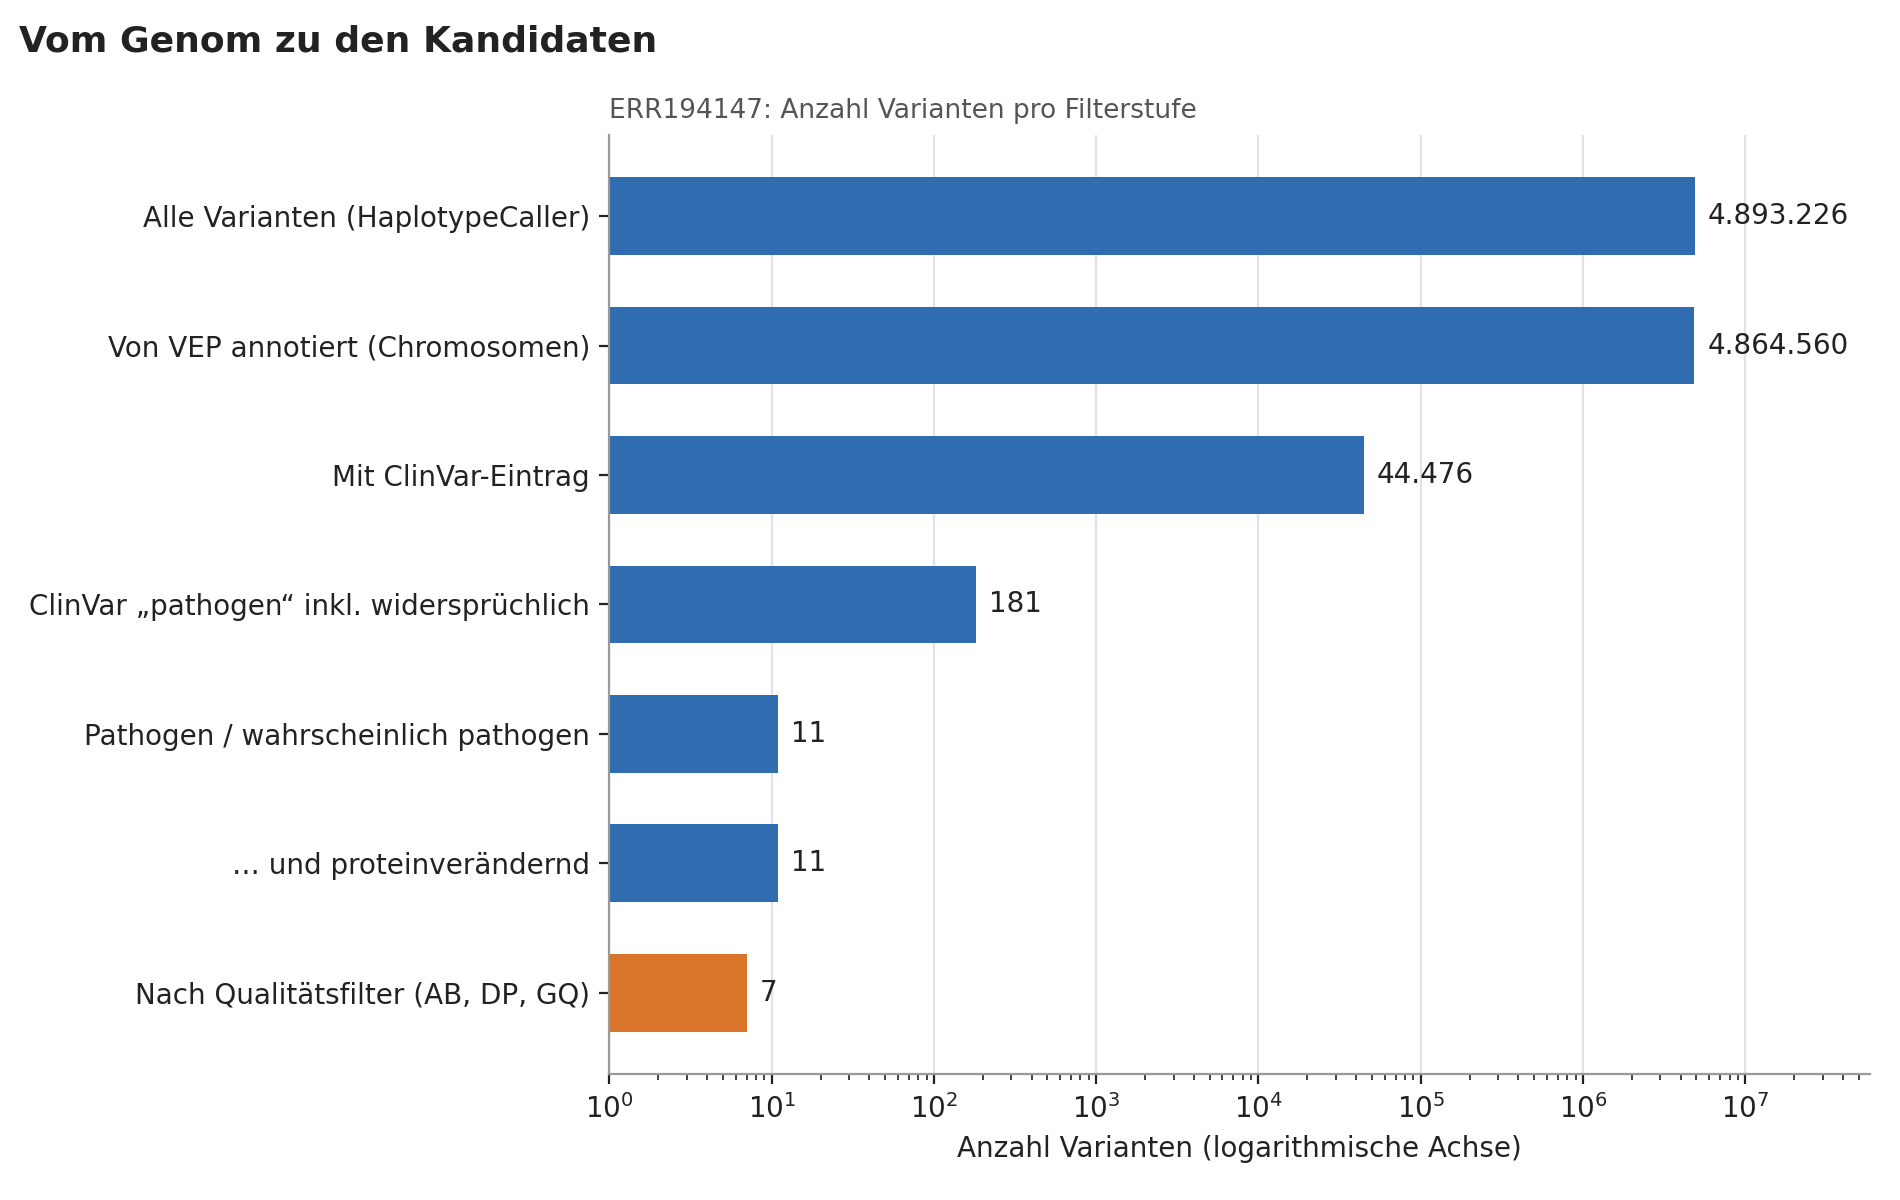
\includegraphics[width=\textwidth]{abbildungen/ERR194147/1_trichter.png}
\caption{Mutter}
\end{subfigure}\hfill
\begin{subfigure}[t]{0.49\columnwidth}
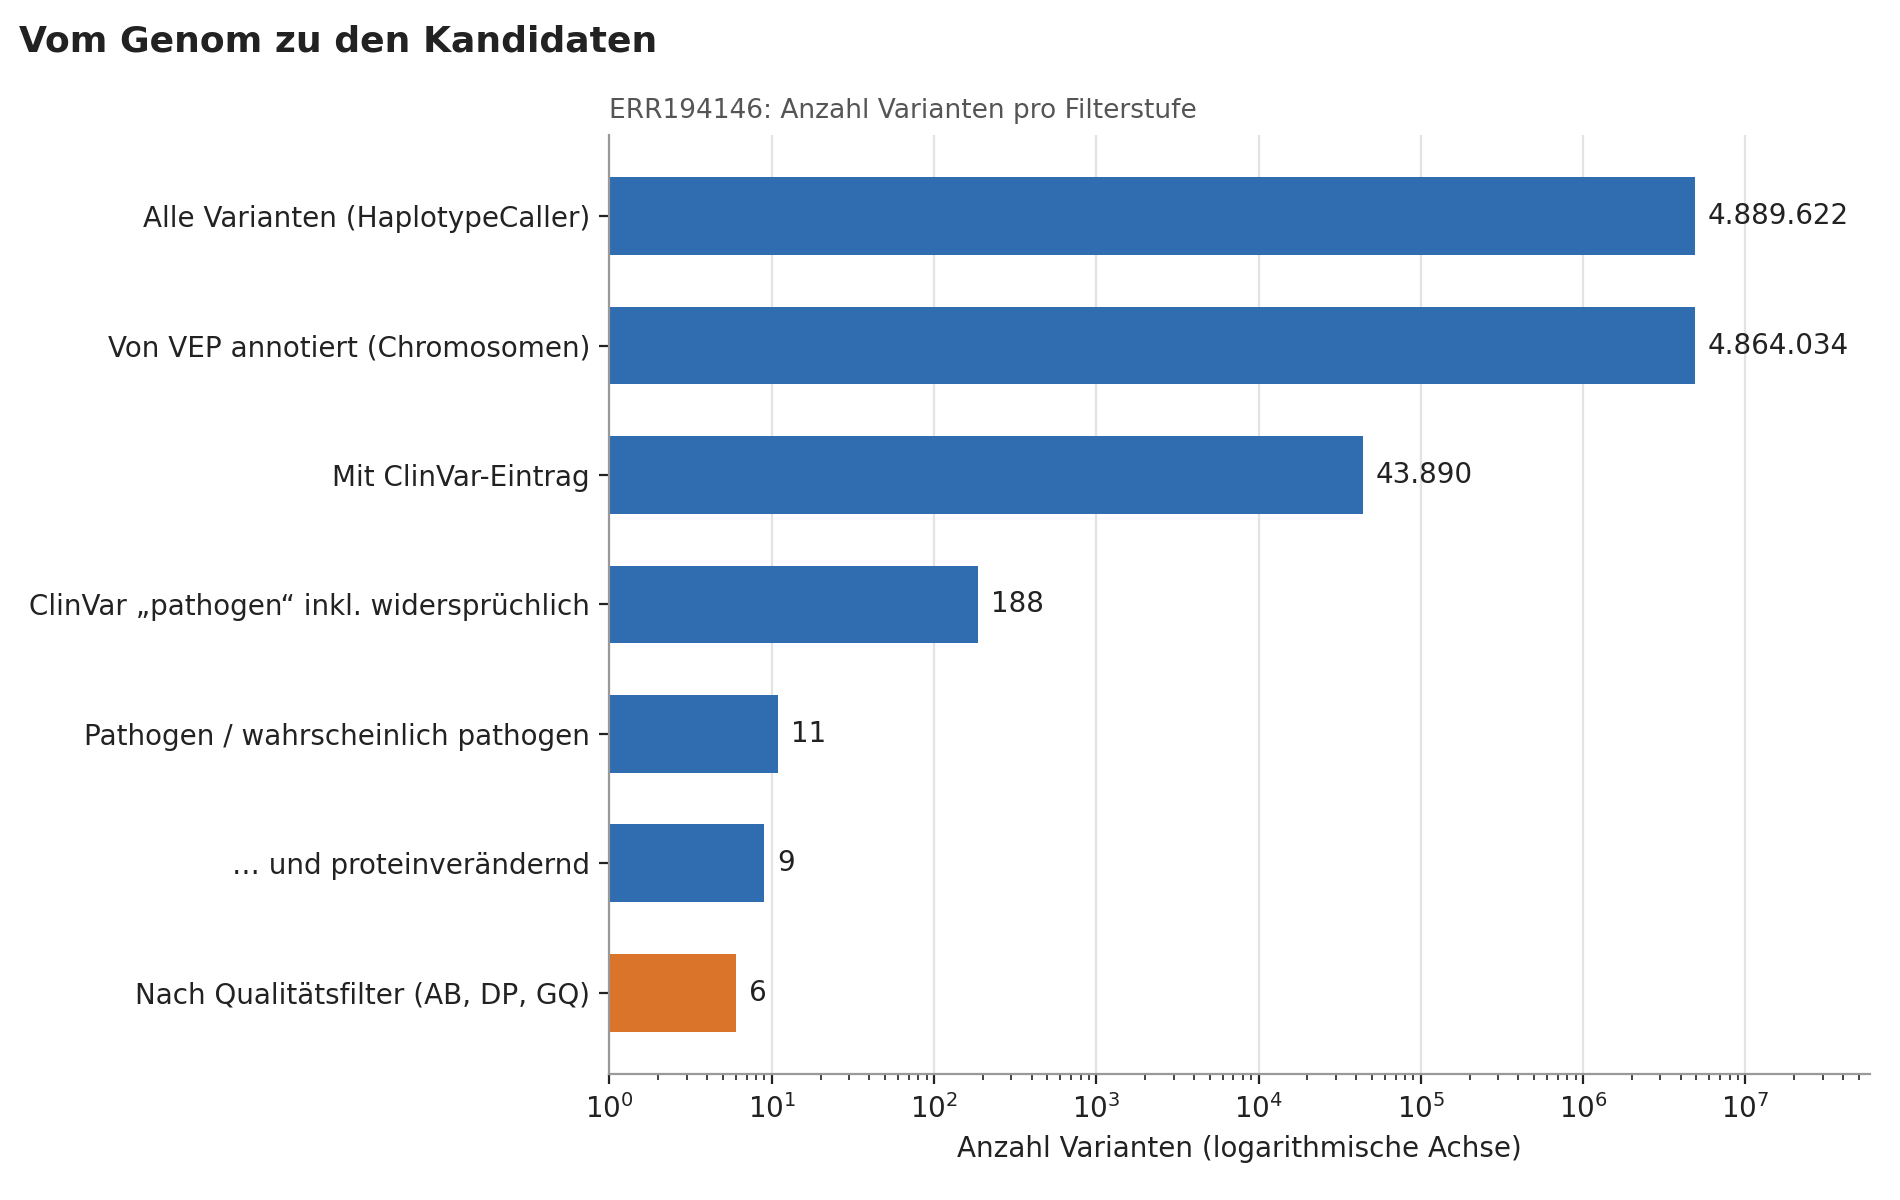
\includegraphics[width=\textwidth]{abbildungen/ERR194146/1_trichter.png}
\caption{Vater}
\end{subfigure}
\caption{Filtertrichter von allen Varianten bis zu den Kandidaten nach Qualit\"atsfilter.}
\label{fig:trichter}
\end{figure}

\begin{figure}[t]
\centering
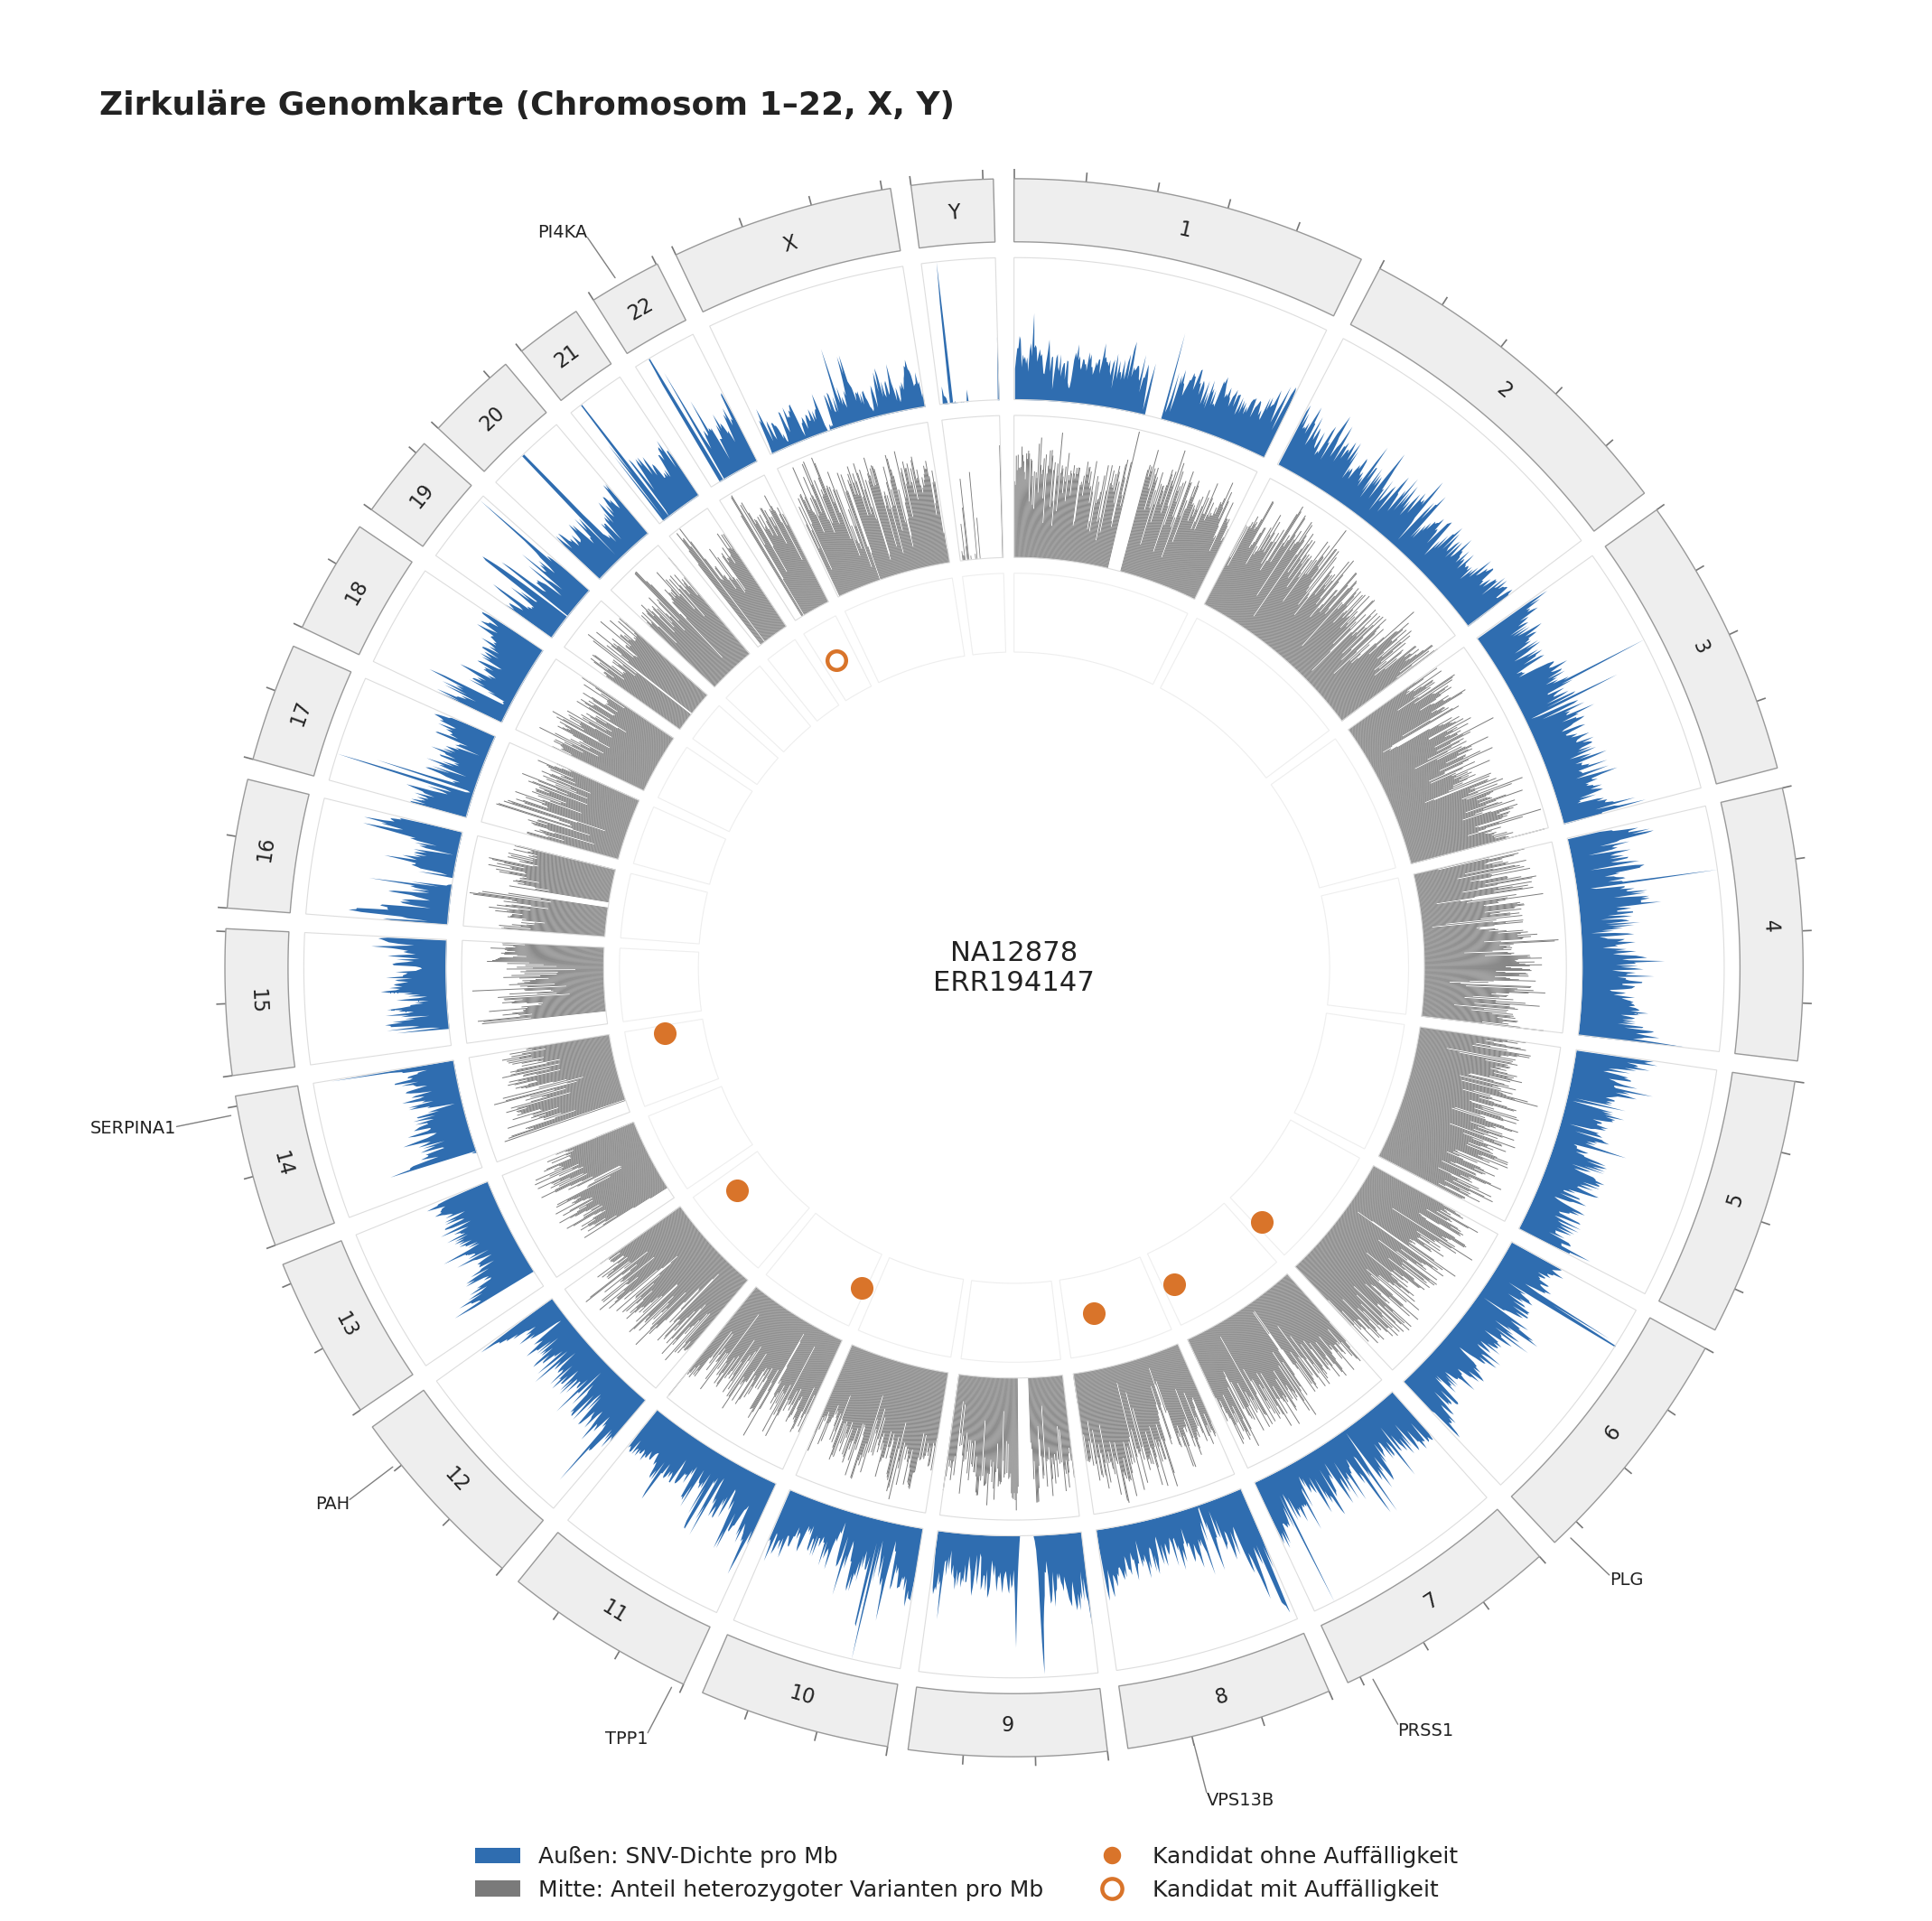
\includegraphics[width=\columnwidth]{abbildungen/ERR194147/7_circos.png}
\caption{Zirkul\"are Genomkarte der Mutter mit SNV-Dichte, Anteil heterozygoter Varianten und Kandidaten (Vater: \texttt{abbildungen/ERR194146/7\_circos.png}).}
\label{fig:circos}
\end{figure}

\subsection{Kandidaten}\label{sec:kand}
Alle verbleibenden Kandidaten sind heterozygot. Tabelle~\ref{tab:kand} zeigt die Ergebnisse nach Qualit\"atspr\"ufung; die Krankheitsangaben und Pr\"ufsterne stammen aus ClinVar und geben dessen Wortlaut wieder. Abbildung~\ref{fig:ab} zeigt die Allelbalance aller Treffer.

\begin{table*}[t]
\centering
\small
\caption{Kandidaten beider Eltern nach Qualit\"atspr\"ufung (GRCh38). AB: Allelbalance; Sterne: ClinVar-Pr\"ufstatus. Krankheitsangaben laut ClinVar, keine Diagnosen.}
\label{tab:kand}
\begin{tabular}{@{}llllrcl@{}}
\toprule
Probe & Gen & Position & Variante / Effekt & AB & Sterne & Klasse\\
\midrule
Mutter & \gene{TPP1} & 11:6617154 & C$>$T, Spleißakzeptor & 0,66 & 2 & belastbar\\
 & \gene{PAH} & 12:102840474 & T$>$C, Missense & 0,61 & 3 & belastbar\\
 & \gene{PLG} & 6:160706469 & A$>$G, Missense & 0,39 & 2 & belastbar\\
 & \gene{PRSS1} & 7:142750561 & C$>$T & 0,32 & 2 & unsicher\\
 & \gene{SERPINA1} & 14:94379549 & A$>$AG, Frameshift & 0,17 & 1 & unsicher\\
 & \gene{VPS13B} & 8:99832366 & TAGTA$>$T, Spleißakzeptor & 0,18 & 1 & unsicher\\
 & \gene{PI4KA} & 22:20709921 & TTGTC$>$T, Frameshift & 0,10 & 2 & unsicher\\
\addlinespace
Vater & \gene{POLG} & 15:89327201 & C$>$T & 0,53 & 2 & belastbar\\
 & \gene{CCDC40} & 17:80039965 & GC$>$G, Frameshift & 0,62 & 2 & belastbar\\
 & \gene{CFTR} & 7:117587738 & G$>$A, Spleißakzeptor & 0,47 & 4 & belastbar\\
 & \gene{CLCN1} & 7:143351678 & C$>$T, Stop gained & 0,61 & 2 & belastbar\\
 & \gene{LAMB2} & 3:49132597 & T$>$G, Missense & 0,28 & 0 & unsicher\\
 & \gene{SERPINA1} & 14:94379549 & A$>$AG, Frameshift & 0,13 & 1 & unsicher\\
\bottomrule
\end{tabular}
\end{table*}

\paragraph{Belastbare Kandidaten.} Bei der Mutter sind \gene{TPP1}, \gene{PAH} und \gene{PLG} belastbar, beim Vater \gene{POLG}, \gene{CCDC40}, \gene{CFTR} und \gene{CLCN1}. Der \gene{CFTR}-Eintrag besitzt mit vier Sternen die h\"ochste Absicherung in ClinVar. Die Krankheitsangaben laut ClinVar lauten \gene{TPP1}: TPP1-related disorder, \gene{PAH}: Hyperphenylalaninemia, \gene{CFTR}: Cystic fibrosis, \gene{CCDC40}: Primary ciliary dyskinesia und \gene{CLCN1}: Skeletal muscle channelopathy. \gene{PLG}~(Plasminogen) und \gene{POLG}~(Sensory ataxic neuropathy, dysarthria, and ophthalmoparesis) sind ebenfalls ClinVar-Eintr\"age; die Vererbung h\"angt bei diesen Genen vom Krankheitsbild ab.

\paragraph{Unsichere Kandidaten.} Alle unsicheren Treffer haben niedrige Allelbalance. Bei \gene{PRSS1} (AB 0,32) liegt der Locus in einer Region mit Paralogen (\gene{PRSS2}, \gene{PRSS3}); die Mapping-Qualit\"at ist dort eingeschr\"ankt. Bei \gene{VPS13B} st\"utzen nur drei Alt-Reads (Tiefe 17) die Deletion. Bei \gene{PI4KA} haben knapp 19~\% der Reads am Locus eine niedrige Mapping-Qualit\"at; die Region enth\"alt Pseudogene (22q11.2), und QD ist mit 1,12 niedrig. Bei \gene{LAMB2} (Vater) sind QD 1,04, SOR 4,97 und FS 44,9 auff\"allig, bei \gene{SERPINA1} erh\"ohte SOR- und FS-Werte (Mutter: FS 34,6, SOR 4,97). Diese Eintr\"age sollten ohne unabh\"angige Best\"atigung nicht als echte Varianten betrachtet werden.

\paragraph{Verworfene Treffer.} Als Artefaktverdacht wurden bei der Mutter \gene{TUBB8} (AB 0,14, subtelomerisch), zwei Positionen in \gene{CNN2} (AB 0,20 und 0,17, GC-reiche Region) und eine zweite \gene{PRSS1}-Position (AB 0,12) verworfen, beim Vater zwei Positionen in \gene{CNN2} (AB 0,13) und \gene{PRSS1} 7:142750561 (AB 0,20).

\begin{figure*}[t]
\centering
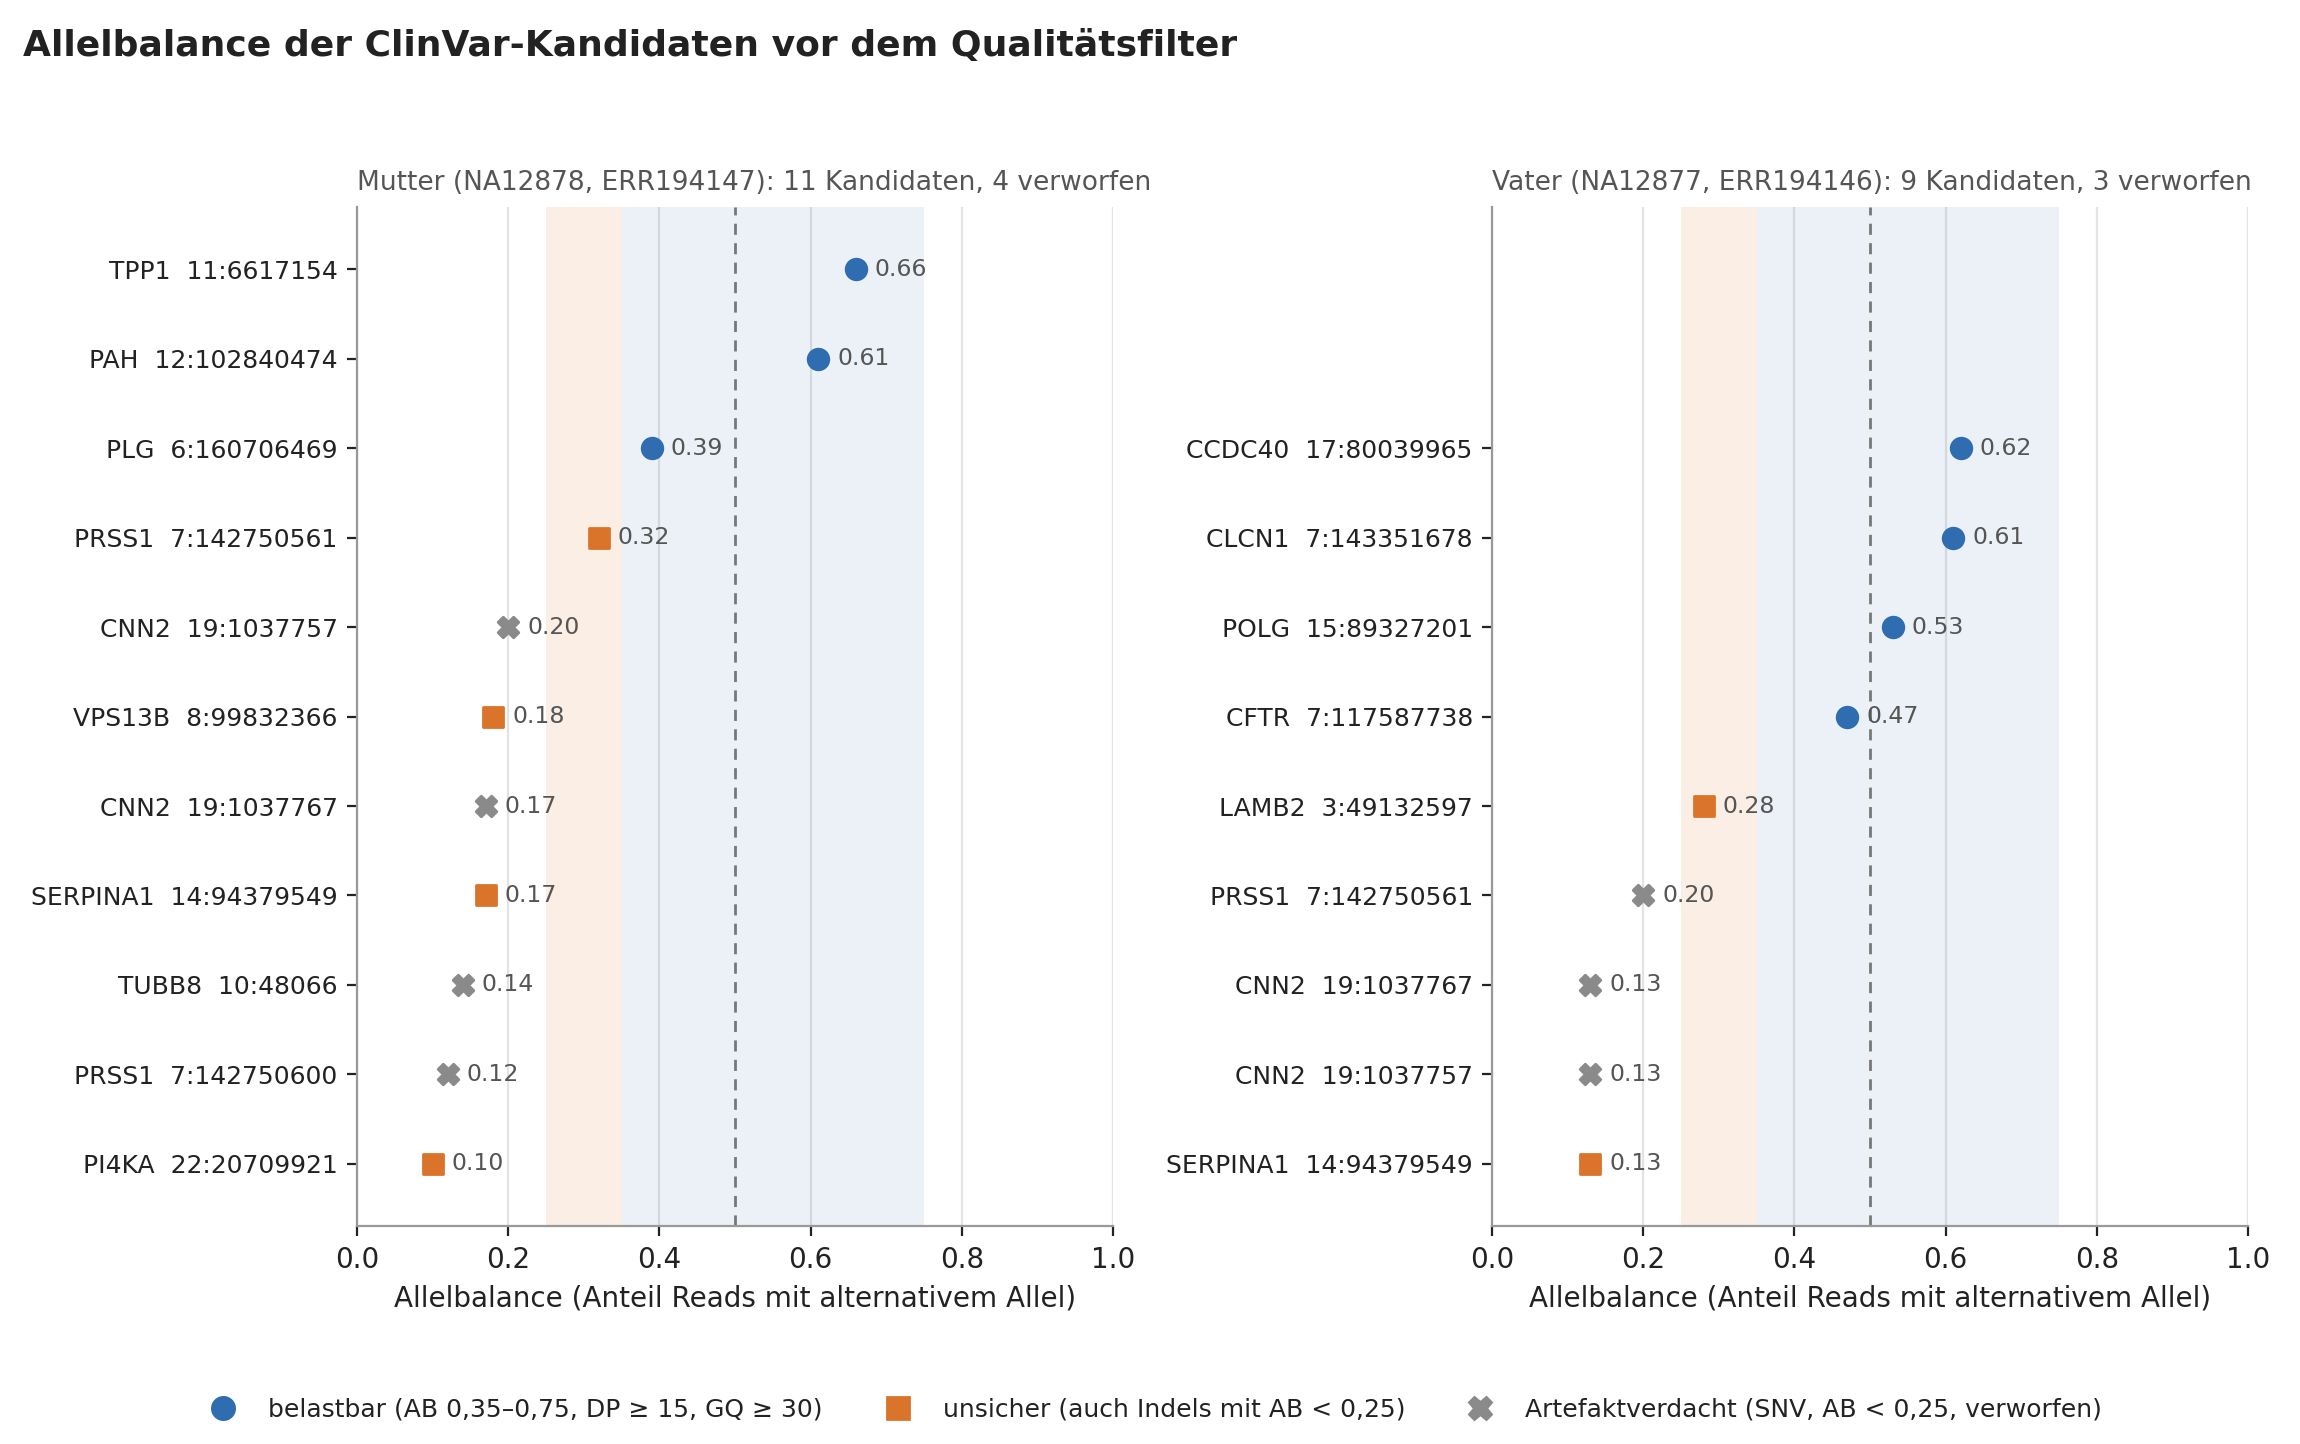
\includegraphics[width=0.7\textwidth]{abbildungen/11_allelbalance_eltern.png}
\caption{Allelbalance der Treffer beider Eltern, farblich nach Qualit\"atsklasse. Heterozygote Varianten liegen bei etwa 0,5; Indels sind wegen verzerrter AD-Werte gesondert behandelt.}
\label{fig:ab}
\end{figure*}

\begin{figure*}[t]
\centering
\begin{subfigure}[t]{0.48\textwidth}
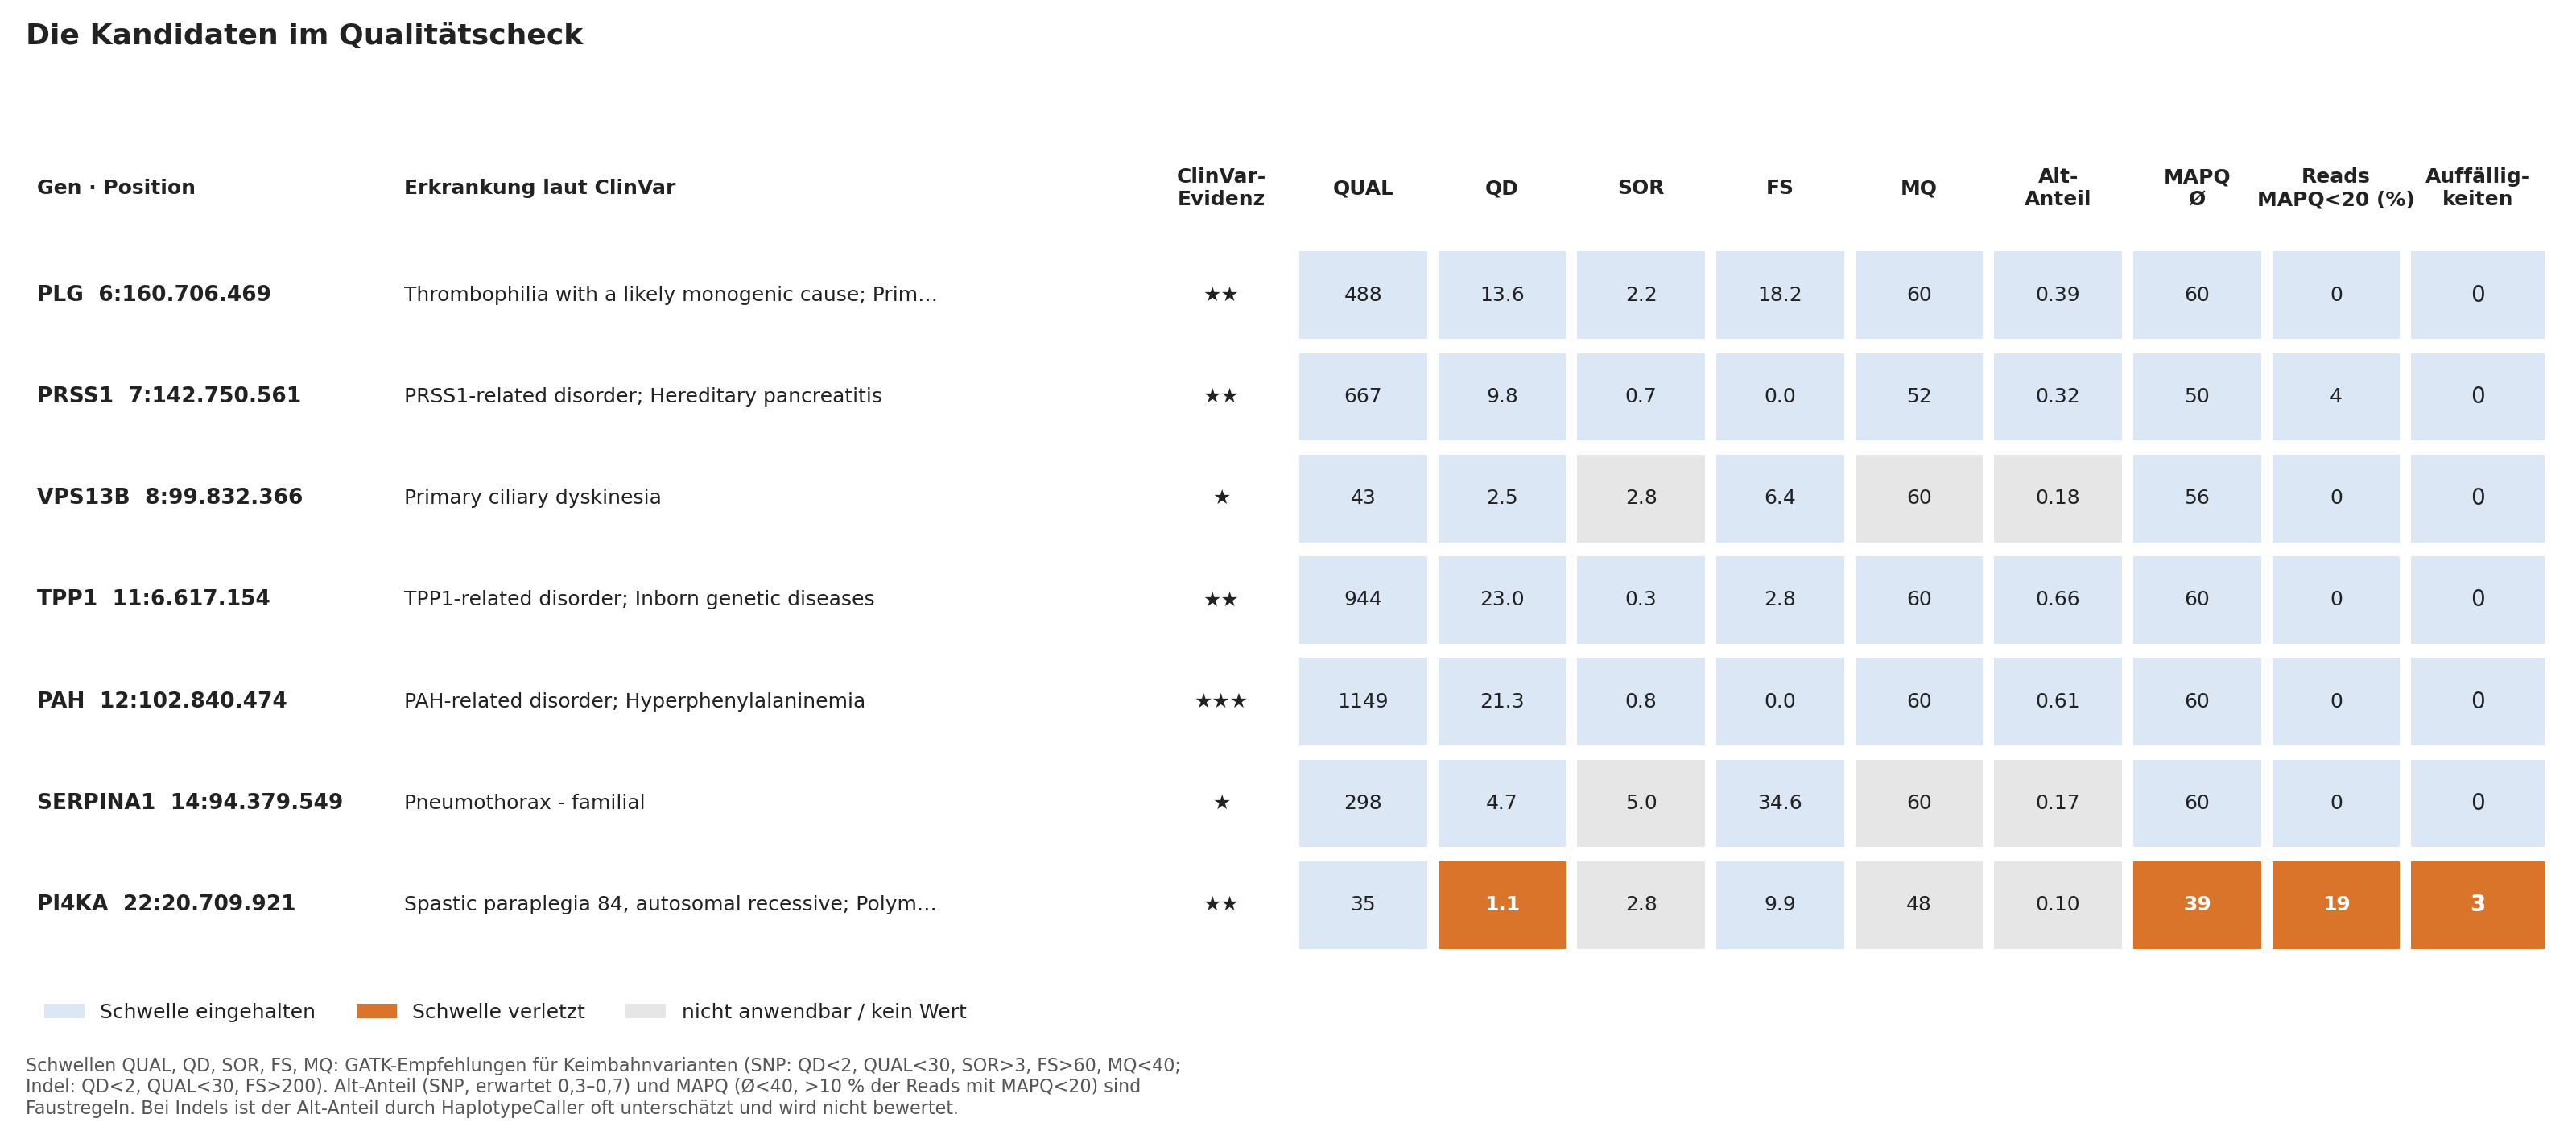
\includegraphics[width=\textwidth]{abbildungen/ERR194147/6_kandidaten_qualitaet.png}
\caption{Mutter (NA12878)}
\end{subfigure}\hfill
\begin{subfigure}[t]{0.48\textwidth}
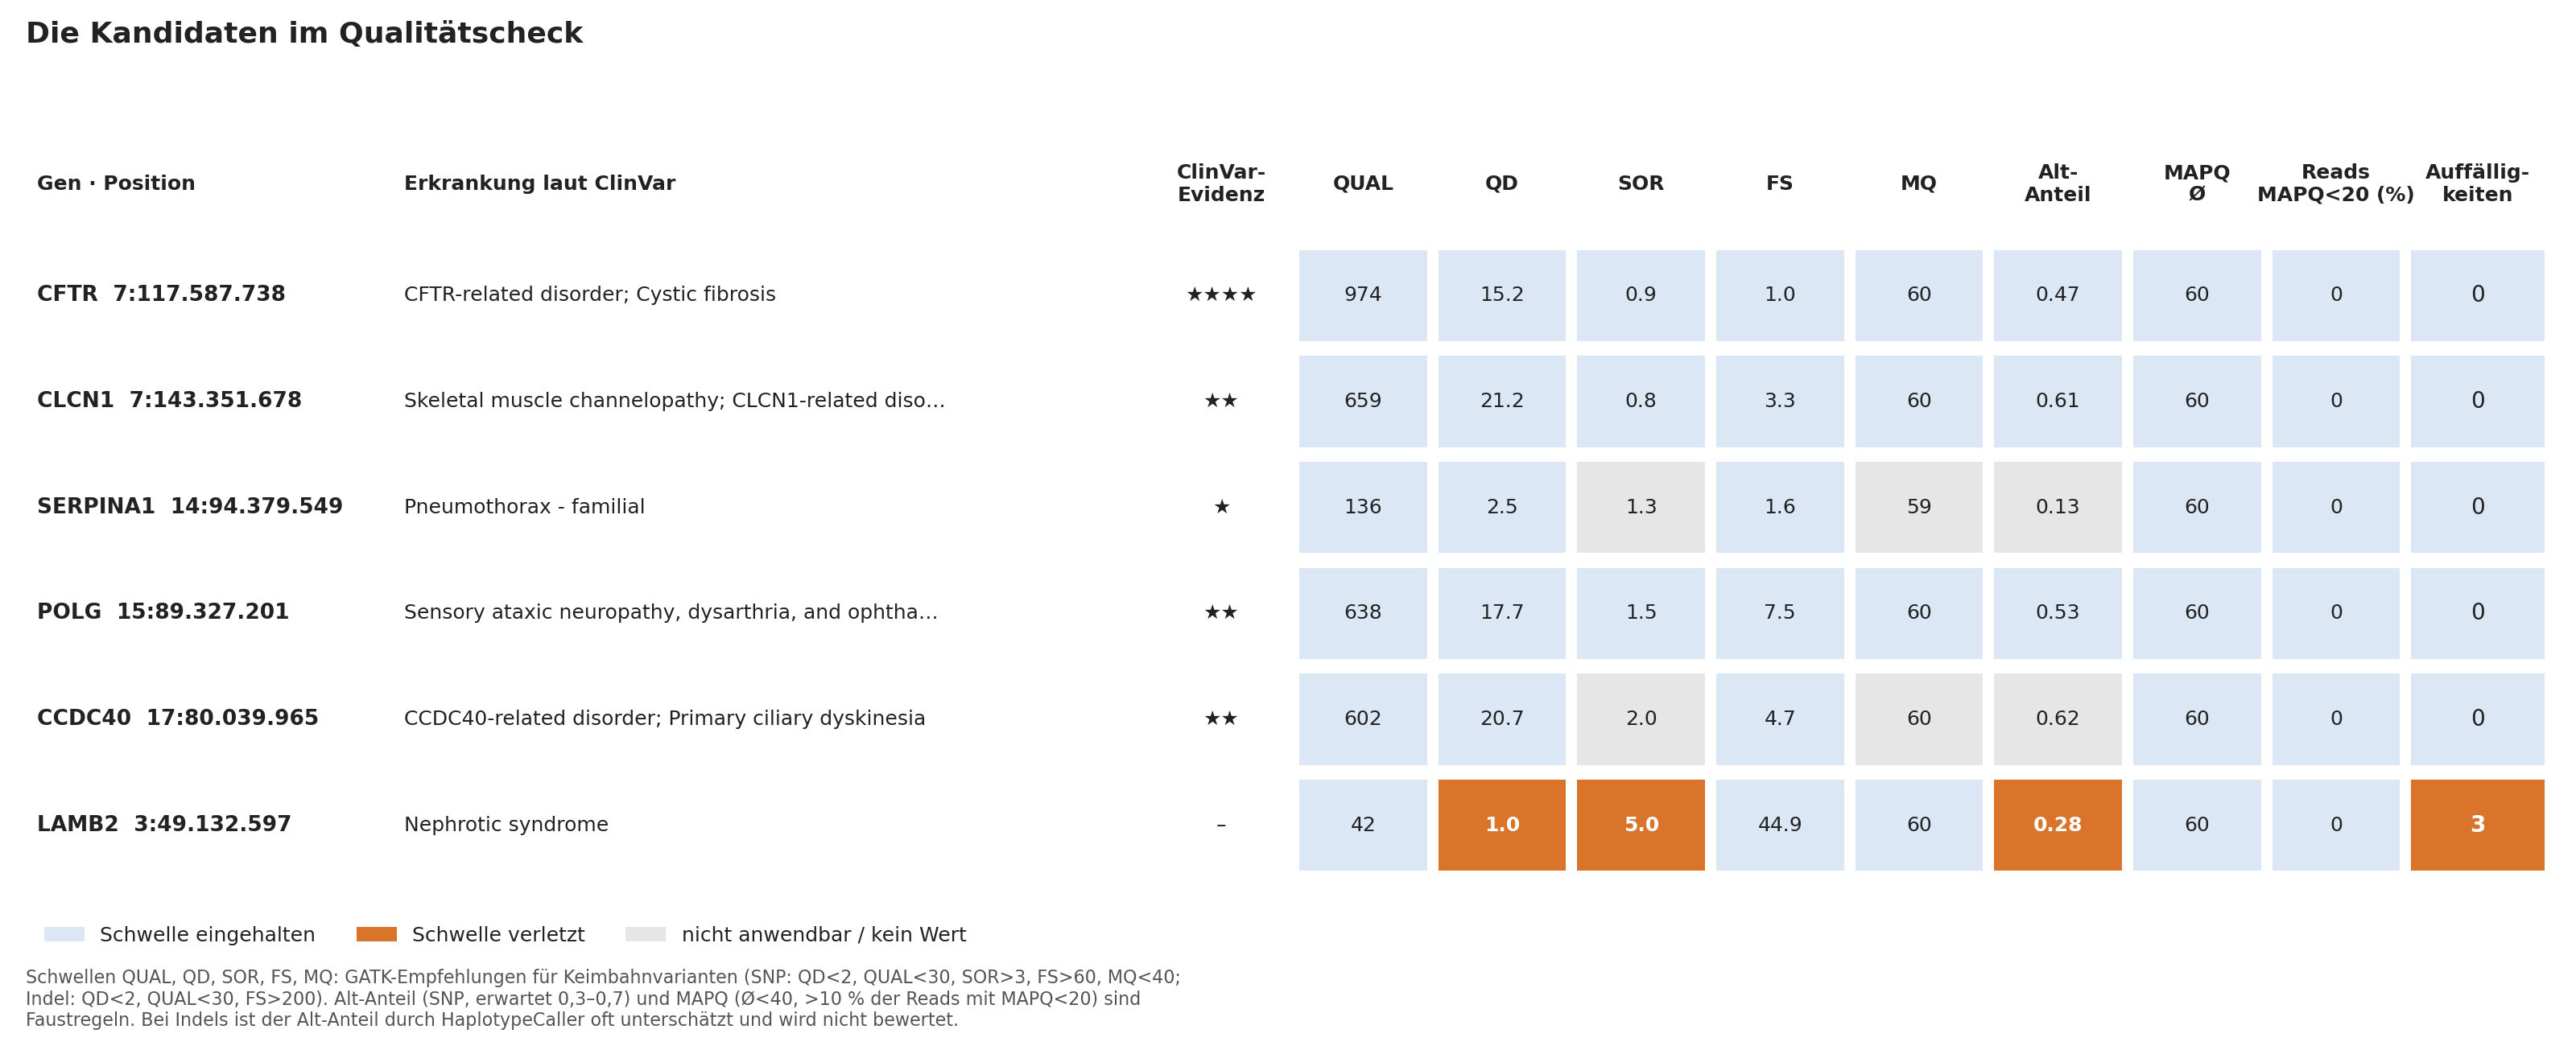
\includegraphics[width=\textwidth]{abbildungen/ERR194146/6_kandidaten_qualitaet.png}
\caption{Vater (NA12877)}
\end{subfigure}
\caption{Qualit\"atswerte der Kandidaten.}
\label{fig:qual}
\end{figure*}

\subsection{Vergleich der Eltern}
Gemeinsam in beiden Genomen erscheint nur \gene{SERPINA1}, und zwar als dieselbe Variante (14:94379549 A$>$AG) mit niedriger Allelbalance (0,17 bzw.\ 0,13). Bei diesem Eintrag stimmen zwei Dinge nicht zu einem echten Befund: Die Allelbalance liegt weit unter 0,5, und in den Roh-Alignments konnte ich die Insertion nicht best\"atigen. Ein Gleiches gilt f\"ur \gene{PRSS1} 7:142750561, das beim Vater verworfen und bei der Mutter nur als unsicher eingestuft wurde, und f\"ur \gene{CNN2}, das in beiden Proben im Artefaktbereich liegt. Dass dieselben Positionen in beiden unabh\"angigen Genomen auftreten, spricht eher f\"ur einen systematischen Mapping- oder Calling-Artefakt als f\"ur eine echte gemeinsame Variante; ein Abgleich mit Populationsfrequenzen (gnomAD) steht noch aus. Das ClinVar-Krankheitsbild des \gene{SERPINA1}-Eintrags (Pneumothorax -- familial) passt zudem nicht zu dem, was man bei diesem Gen erwarten w\"urde, und sollte nicht als Alpha-1-Antitrypsin-Mangel gelesen werden.

Unter den belastbaren Kandidaten gibt es daher kein gemeinsames Gen. Die Mutter tr\"agt Varianten in \gene{TPP1}, \gene{PAH} und \gene{PLG}, der Vater in \gene{POLG}, \gene{CCDC40}, \gene{CFTR} und \gene{CLCN1}. F\"ur klassisch rezessive Erkrankungen wie \gene{TPP1}, \gene{PAH}, \gene{CFTR} und \gene{CCDC40} bedeutet das: Ein gemeinsames Kind h\"atte f\"ur jede dieser Varianten, die nur ein Elternteil tr\"agt, eine Wahrscheinlichkeit von 50~\%, Tr\"ager zu sein, aber kein erh\"ohtes Risiko, selbst zu erkranken, da die zweite Kopie aus dem anderen Elternteil unauff\"allig w\"are. Nur wenn beide Eltern dieselbe rezessive Variante (oder zwei Varianten im selben Gen) tragen, ergibt sich das 25-\%-Risiko mit 50~\% Tr\"agern und 25~\% ohne Variante. Der Erbgang ist in den Tabellen nicht enthalten und m\"usste f\"ur jedes Gen in der Literatur nachgeschlagen werden.

\section{Diskussion}
Die beiden Genome sind technisch vergleichbar (Tab.~\ref{tab:qc}, \ref{tab:var}); Mapping-Rate, Duplikationsrate, Ti/Tv und Het/Hom-Verh\"altnis liegen im erwarteten Bereich. Das wichtigste inhaltliche Ergebnis ist, dass der strenge ClinVar-Filter ohne Qualit\"atspr\"ufung ein falsches Bild gezeichnet h\"atte: Von je 11 Treffern blieben nach Pr\"ufung nur 7 bzw.\ 6, und nur 3 bzw.\ 4 sind belastbar. Mehrere der verworfenen Treffer liegen in Regionen, die f\"ur Mapping-Probleme bekannt sind (Paraloge, Pseudogene, GC-reiche oder subtelomerische Bereiche). Ein ungefilterter Variantensatz f\"uhrt hier also zu Scheintreffern; ein Hard Filter oder VQSR sowie BQSR w\"aren in einer produktiven Pipeline erforderlich.

Die Allelbalance ist ein pragmatisches, aber grobes Kriterium. Sie ist bei Indels verzerrt, weshalb diese bei niedriger AB nur als unsicher und nicht als Artefakt gelten. Die Einstufung \emph{unsicher} hei\ss t deshalb nicht, dass die Variante falsch ist, sondern dass die Daten sie nicht ausreichend belegen.

\section{Einschr\"ankungen}
\begin{itemize}
\item \textbf{Keine Validierung gegen ein Truth Set.} Sensitivit\"at und Pr\"azision der Variantenbestimmung wurden nicht quantifiziert. Ein Vergleich mit den Platinum-Genomes- bzw.\ GIAB-Referenzcalls \citep{eberle2017,zook2014} ist geplant.
\item Kein Variantenfilter (VQSR/Hard Filter), kein BQSR; die Schwellen des Kandidatenfilters sind nicht kalibriert.
\item \gene{SERPINA1} wurde in den Roh-Alignments nicht best\"atigt; die Hinweise auf systematische Artefakte (\gene{PRSS1}, \gene{CNN2}, \gene{SERPINA1} in beiden Proben) sind nicht durch Populationsfrequenzen abgesichert.
\item Etwa 0,6~\% der gerufenen Varianten tauchen in der VEP-Ausgabe nicht auf; die Ursache ist nicht vollst\"andig gekl\"art.
\item ClinVar-Klassifikationen sind teils \"alter oder nur von einem Einreicher abgesichert; Sterne und Krankheitsbezeichnungen sind hier w\"ortlich wiedergegeben und nicht fachlich neu bewertet.
\item Es wurden nur SNVs und kleine Indels betrachtet; Strukturvarianten, Kopienzahl und Mitochondrium wurden nicht ausgewertet.
\item Die Ergebnisse sind keine Diagnosen und ersetzen keine humangenetische Beratung.
\end{itemize}

\section{Ausblick}
Als n\"achste Schritte sind eine Validierung gegen das Truth Set (z.\,B.\ mit rtg vcfeval oder hap.py, mit angepassten Chromosomennamen), ein Variantenfilter nach GATK-Empfehlung, die Pr\"ufung der unsicheren Treffer in IGV und der Abgleich mit Populationsfrequenzen vorgesehen.

\section{Schlussfolgerung}
Die Pipeline verarbeitet zwei Gesamtgenome reproduzierbar von den Rohdaten bis zu annotierten Kandidaten. Die Qualit\"atspr\"ufung zeigt, dass ein strenger ClinVar-Filter allein nicht ausreicht: Erst die Kombination mit Allelbalance, Tiefe und Genotypqualit\"at trennt belastbare Treffer von Mapping-Artefakten. Im Elternvergleich ergab sich kein Gen mit belastbaren Varianten bei beiden Eltern. Alle Aussagen sind ClinVar-Annotationen ohne Diagnosewert.

\section*{Datenverf\"ugbarkeit}
Die Rohdaten sind \"offentlich verf\"ugbar (ENA: ERR194147, ERR194146). Code und Konfiguration der Pipeline stehen im Projektverzeichnis bzw.\ im zugeh\"origen GitHub-Repository.

\bibliographystyle{plainnat}
\bibliography{literatur}
\end{document}
